\documentclass[twoside]{book}

% Packages required by doxygen
\usepackage{fixltx2e}
\usepackage{calc}
\usepackage{doxygen}
\usepackage[export]{adjustbox} % also loads graphicx
\usepackage{graphicx}
\usepackage[utf8]{inputenc}
\usepackage{makeidx}
\usepackage{multicol}
\usepackage{multirow}
\PassOptionsToPackage{warn}{textcomp}
\usepackage{textcomp}
\usepackage[nointegrals]{wasysym}
\usepackage[table]{xcolor}

% Font selection
\usepackage[T1]{fontenc}
\usepackage[scaled=.90]{helvet}
\usepackage{courier}
\usepackage{amssymb}
\usepackage{sectsty}
\renewcommand{\familydefault}{\sfdefault}
\allsectionsfont{%
  \fontseries{bc}\selectfont%
  \color{darkgray}%
}
\renewcommand{\DoxyLabelFont}{%
  \fontseries{bc}\selectfont%
  \color{darkgray}%
}
\newcommand{\+}{\discretionary{\mbox{\scriptsize$\hookleftarrow$}}{}{}}

% Page & text layout
\usepackage{geometry}
\geometry{%
  a4paper,%
  top=2.5cm,%
  bottom=2.5cm,%
  left=2.5cm,%
  right=2.5cm%
}
\tolerance=750
\hfuzz=15pt
\hbadness=750
\setlength{\emergencystretch}{15pt}
\setlength{\parindent}{0cm}
\setlength{\parskip}{3ex plus 2ex minus 2ex}
\makeatletter
\renewcommand{\paragraph}{%
  \@startsection{paragraph}{4}{0ex}{-1.0ex}{1.0ex}{%
    \normalfont\normalsize\bfseries\SS@parafont%
  }%
}
\renewcommand{\subparagraph}{%
  \@startsection{subparagraph}{5}{0ex}{-1.0ex}{1.0ex}{%
    \normalfont\normalsize\bfseries\SS@subparafont%
  }%
}
\makeatother

% Headers & footers
\usepackage{fancyhdr}
\pagestyle{fancyplain}
\fancyhead[LE]{\fancyplain{}{\bfseries\thepage}}
\fancyhead[CE]{\fancyplain{}{}}
\fancyhead[RE]{\fancyplain{}{\bfseries\leftmark}}
\fancyhead[LO]{\fancyplain{}{\bfseries\rightmark}}
\fancyhead[CO]{\fancyplain{}{}}
\fancyhead[RO]{\fancyplain{}{\bfseries\thepage}}
\fancyfoot[LE]{\fancyplain{}{}}
\fancyfoot[CE]{\fancyplain{}{}}
\fancyfoot[RE]{\fancyplain{}{\bfseries\scriptsize Generated by Doxygen }}
\fancyfoot[LO]{\fancyplain{}{\bfseries\scriptsize Generated by Doxygen }}
\fancyfoot[CO]{\fancyplain{}{}}
\fancyfoot[RO]{\fancyplain{}{}}
\renewcommand{\footrulewidth}{0.4pt}
\renewcommand{\chaptermark}[1]{%
  \markboth{#1}{}%
}
\renewcommand{\sectionmark}[1]{%
  \markright{\thesection\ #1}%
}

% Indices & bibliography
\usepackage{natbib}
\usepackage[titles]{tocloft}
\setcounter{tocdepth}{3}
\setcounter{secnumdepth}{5}
\makeindex

% Hyperlinks (required, but should be loaded last)
\usepackage{ifpdf}
\ifpdf
  \usepackage[pdftex,pagebackref=true]{hyperref}
\else
  \usepackage[ps2pdf,pagebackref=true]{hyperref}
\fi
\hypersetup{%
  colorlinks=true,%
  linkcolor=blue,%
  citecolor=blue,%
  unicode%
}

% Custom commands
\newcommand{\clearemptydoublepage}{%
  \newpage{\pagestyle{empty}\cleardoublepage}%
}

\usepackage{caption}
\captionsetup{labelsep=space,justification=centering,font={bf},singlelinecheck=off,skip=4pt,position=top}

%===== C O N T E N T S =====

\begin{document}

% Titlepage & ToC
\hypersetup{pageanchor=false,
             bookmarksnumbered=true,
             pdfencoding=unicode
            }
\pagenumbering{alph}
\begin{titlepage}
\vspace*{7cm}
\begin{center}%
{\Large Agenda }\\
\vspace*{1cm}
{\large Generated by Doxygen 1.8.14}\\
\end{center}
\end{titlepage}
\clearemptydoublepage
\pagenumbering{roman}
\tableofcontents
\clearemptydoublepage
\pagenumbering{arabic}
\hypersetup{pageanchor=true}

%--- Begin generated contents ---
\chapter{Hierarchical Index}
\section{Class Hierarchy}
This inheritance list is sorted roughly, but not completely, alphabetically\+:\begin{DoxyCompactList}
\item \contentsline{section}{Source.\+core.\+collection.\+Collection}{\pageref{classSource_1_1core_1_1collection_1_1Collection}}{}
\item \contentsline{section}{Source.\+core.\+presence.\+Presence}{\pageref{classSource_1_1core_1_1presence_1_1Presence}}{}
\item \contentsline{section}{property}{\pageref{classproperty}}{}
\begin{DoxyCompactList}
\item \contentsline{section}{Source.\+core.\+dataproperty.\+Data\+Owner\+Property}{\pageref{classSource_1_1core_1_1dataproperty_1_1DataOwnerProperty}}{}
\item \contentsline{section}{Source.\+core.\+dataproperty.\+Data\+Property}{\pageref{classSource_1_1core_1_1dataproperty_1_1DataProperty}}{}
\end{DoxyCompactList}
\item \contentsline{section}{Source.\+core.\+dataweak.\+Weak\+Refered}{\pageref{classSource_1_1core_1_1dataweak_1_1WeakRefered}}{}
\begin{DoxyCompactList}
\item \contentsline{section}{Source.\+core.\+data.\+Data}{\pageref{classSource_1_1core_1_1data_1_1Data}}{}
\begin{DoxyCompactList}
\item \contentsline{section}{Source.\+core.\+account.\+Account}{\pageref{classSource_1_1core_1_1account_1_1Account}}{}
\item \contentsline{section}{Source.\+core.\+agenda.\+Agenda}{\pageref{classSource_1_1core_1_1agenda_1_1Agenda}}{}
\item \contentsline{section}{Source.\+core.\+event.\+Event}{\pageref{classSource_1_1core_1_1event_1_1Event}}{}
\item \contentsline{section}{Source.\+core.\+group.\+Group}{\pageref{classSource_1_1core_1_1group_1_1Group}}{}
\item \contentsline{section}{Source.\+core.\+notification.\+Notification}{\pageref{classSource_1_1core_1_1notification_1_1Notification}}{}
\item \contentsline{section}{Source.\+core.\+resource.\+Resource}{\pageref{classSource_1_1core_1_1resource_1_1Resource}}{}
\item \contentsline{section}{Source.\+core.\+user.\+User}{\pageref{classSource_1_1core_1_1user_1_1User}}{}
\end{DoxyCompactList}
\item \contentsline{section}{Source.\+core.\+dataproxy.\+Data\+Proxy}{\pageref{classSource_1_1core_1_1dataproxy_1_1DataProxy}}{}
\end{DoxyCompactList}
\item \contentsline{section}{Source.\+core.\+dataweak.\+Weak\+Ref\+Set}{\pageref{classSource_1_1core_1_1dataweak_1_1WeakRefSet}}{}
\end{DoxyCompactList}

\chapter{Class Index}
\section{Class List}
Here are the classes, structs, unions and interfaces with brief descriptions\+:\begin{DoxyCompactList}
\item\contentsline{section}{\mbox{\hyperlink{classSource_1_1core_1_1account_1_1Account}{Source.\+core.\+account.\+Account}} }{\pageref{classSource_1_1core_1_1account_1_1Account}}{}
\item\contentsline{section}{\mbox{\hyperlink{classSource_1_1core_1_1agenda_1_1Agenda}{Source.\+core.\+agenda.\+Agenda}} }{\pageref{classSource_1_1core_1_1agenda_1_1Agenda}}{}
\item\contentsline{section}{\mbox{\hyperlink{classSource_1_1core_1_1collection_1_1Collection}{Source.\+core.\+collection.\+Collection}} \\*\mbox{\hyperlink{classSource_1_1core_1_1collection_1_1Collection}{Collection}} de toutes les données du système }{\pageref{classSource_1_1core_1_1collection_1_1Collection}}{}
\item\contentsline{section}{\mbox{\hyperlink{classSource_1_1core_1_1data_1_1Data}{Source.\+core.\+data.\+Data}} }{\pageref{classSource_1_1core_1_1data_1_1Data}}{}
\item\contentsline{section}{\mbox{\hyperlink{classSource_1_1core_1_1dataproperty_1_1DataOwnerProperty}{Source.\+core.\+dataproperty.\+Data\+Owner\+Property}} }{\pageref{classSource_1_1core_1_1dataproperty_1_1DataOwnerProperty}}{}
\item\contentsline{section}{\mbox{\hyperlink{classSource_1_1core_1_1dataproperty_1_1DataProperty}{Source.\+core.\+dataproperty.\+Data\+Property}} }{\pageref{classSource_1_1core_1_1dataproperty_1_1DataProperty}}{}
\item\contentsline{section}{\mbox{\hyperlink{classSource_1_1core_1_1dataproxy_1_1DataProxy}{Source.\+core.\+dataproxy.\+Data\+Proxy}} }{\pageref{classSource_1_1core_1_1dataproxy_1_1DataProxy}}{}
\item\contentsline{section}{\mbox{\hyperlink{classSource_1_1core_1_1event_1_1Event}{Source.\+core.\+event.\+Event}} }{\pageref{classSource_1_1core_1_1event_1_1Event}}{}
\item\contentsline{section}{\mbox{\hyperlink{classSource_1_1core_1_1group_1_1Group}{Source.\+core.\+group.\+Group}} }{\pageref{classSource_1_1core_1_1group_1_1Group}}{}
\item\contentsline{section}{\mbox{\hyperlink{classSource_1_1core_1_1notification_1_1Notification}{Source.\+core.\+notification.\+Notification}} }{\pageref{classSource_1_1core_1_1notification_1_1Notification}}{}
\item\contentsline{section}{\mbox{\hyperlink{classSource_1_1core_1_1presence_1_1Presence}{Source.\+core.\+presence.\+Presence}} }{\pageref{classSource_1_1core_1_1presence_1_1Presence}}{}
\item\contentsline{section}{\mbox{\hyperlink{classproperty}{property}} }{\pageref{classproperty}}{}
\item\contentsline{section}{\mbox{\hyperlink{classSource_1_1core_1_1resource_1_1Resource}{Source.\+core.\+resource.\+Resource}} }{\pageref{classSource_1_1core_1_1resource_1_1Resource}}{}
\item\contentsline{section}{\mbox{\hyperlink{classSource_1_1core_1_1user_1_1User}{Source.\+core.\+user.\+User}} }{\pageref{classSource_1_1core_1_1user_1_1User}}{}
\item\contentsline{section}{\mbox{\hyperlink{classSource_1_1core_1_1dataweak_1_1WeakRefered}{Source.\+core.\+dataweak.\+Weak\+Refered}} }{\pageref{classSource_1_1core_1_1dataweak_1_1WeakRefered}}{}
\item\contentsline{section}{\mbox{\hyperlink{classSource_1_1core_1_1dataweak_1_1WeakRefSet}{Source.\+core.\+dataweak.\+Weak\+Ref\+Set}} }{\pageref{classSource_1_1core_1_1dataweak_1_1WeakRefSet}}{}
\end{DoxyCompactList}

\chapter{Class Documentation}
\hypertarget{classSource_1_1core_1_1account_1_1Account}{}\section{Source.\+core.\+account.\+Account Class Reference}
\label{classSource_1_1core_1_1account_1_1Account}\index{Source.\+core.\+account.\+Account@{Source.\+core.\+account.\+Account}}


Inheritance diagram for Source.\+core.\+account.\+Account\+:\nopagebreak
\begin{figure}[H]
\begin{center}
\leavevmode
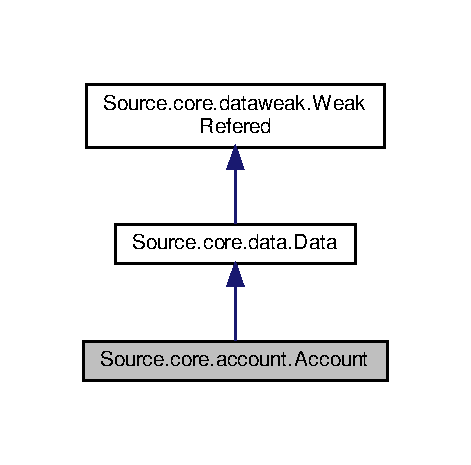
\includegraphics[width=226pt]{classSource_1_1core_1_1account_1_1Account__inherit__graph}
\end{center}
\end{figure}


Collaboration diagram for Source.\+core.\+account.\+Account\+:\nopagebreak
\begin{figure}[H]
\begin{center}
\leavevmode
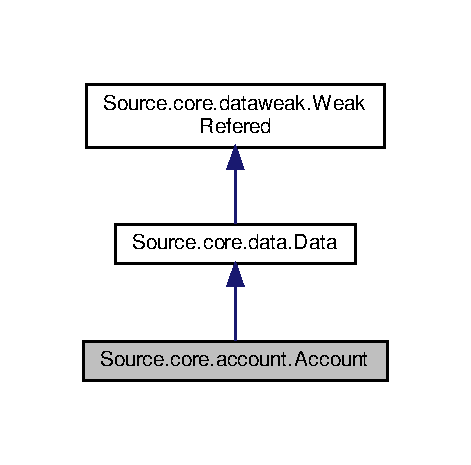
\includegraphics[width=226pt]{classSource_1_1core_1_1account_1_1Account__coll__graph}
\end{center}
\end{figure}
\subsection*{Public Member Functions}
\begin{DoxyCompactItemize}
\item 
def \mbox{\hyperlink{classSource_1_1core_1_1account_1_1Account_aa71293ac376857c39d9fcbac6e0326e3}{\+\_\+\+\_\+init\+\_\+\+\_\+}} (self, \+\_\+id, collection, users, login, mdp, email)
\begin{DoxyCompactList}\small\item\em Création d\textquotesingle{}un compte. \end{DoxyCompactList}\item 
\mbox{\Hypertarget{classSource_1_1core_1_1account_1_1Account_a9c3523f9d004418ecc133edd9609d0ee}\label{classSource_1_1core_1_1account_1_1Account_a9c3523f9d004418ecc133edd9609d0ee}} 
def \mbox{\hyperlink{classSource_1_1core_1_1account_1_1Account_a9c3523f9d004418ecc133edd9609d0ee}{\+\_\+\+\_\+repr\+\_\+\+\_\+}} (self)
\begin{DoxyCompactList}\small\item\em affiche les users d\textquotesingle{}un compte \end{DoxyCompactList}\item 
def \mbox{\hyperlink{classSource_1_1core_1_1account_1_1Account_af7fe8d9e5acb618decb4d24e25df1369}{add\+\_\+user}} (self, user)
\begin{DoxyCompactList}\small\item\em Ajout d\textquotesingle{}un utilisateur au compte. \end{DoxyCompactList}\item 
def \mbox{\hyperlink{classSource_1_1core_1_1account_1_1Account_a6ea6932799b88c2cad17b8c1ce562061}{remove\+\_\+user}} (self, user)
\begin{DoxyCompactList}\small\item\em Suppression d\textquotesingle{}un utilisateur au compte. \end{DoxyCompactList}\end{DoxyCompactItemize}
\subsection*{Public Attributes}
\begin{DoxyCompactItemize}
\item 
\mbox{\Hypertarget{classSource_1_1core_1_1account_1_1Account_ab226de30006271964576c7716c554283}\label{classSource_1_1core_1_1account_1_1Account_ab226de30006271964576c7716c554283}} 
{\bfseries users}
\end{DoxyCompactItemize}
\subsection*{Static Public Attributes}
\begin{DoxyCompactItemize}
\item 
\mbox{\Hypertarget{classSource_1_1core_1_1account_1_1Account_a287c67e1ec615b05edc427326c0760b1}\label{classSource_1_1core_1_1account_1_1Account_a287c67e1ec615b05edc427326c0760b1}} 
{\bfseries login} = \mbox{\hyperlink{classSource_1_1core_1_1dataproperty_1_1DataProperty}{Data\+Property}}(\char`\"{}login\char`\"{})
\item 
\mbox{\Hypertarget{classSource_1_1core_1_1account_1_1Account_ab94bd51e9cc1bbb247aabe7c48b35baf}\label{classSource_1_1core_1_1account_1_1Account_ab94bd51e9cc1bbb247aabe7c48b35baf}} 
{\bfseries mdp} = \mbox{\hyperlink{classSource_1_1core_1_1dataproperty_1_1DataProperty}{Data\+Property}}(\char`\"{}mdp\char`\"{})
\item 
\mbox{\Hypertarget{classSource_1_1core_1_1account_1_1Account_a7b4dd6c4b26008fefc2d6657f8cfc4b0}\label{classSource_1_1core_1_1account_1_1Account_a7b4dd6c4b26008fefc2d6657f8cfc4b0}} 
{\bfseries email} = \mbox{\hyperlink{classSource_1_1core_1_1dataproperty_1_1DataProperty}{Data\+Property}}(\char`\"{}email\char`\"{})
\end{DoxyCompactItemize}


\subsection{Constructor \& Destructor Documentation}
\mbox{\Hypertarget{classSource_1_1core_1_1account_1_1Account_aa71293ac376857c39d9fcbac6e0326e3}\label{classSource_1_1core_1_1account_1_1Account_aa71293ac376857c39d9fcbac6e0326e3}} 
\index{Source\+::core\+::account\+::\+Account@{Source\+::core\+::account\+::\+Account}!\+\_\+\+\_\+init\+\_\+\+\_\+@{\+\_\+\+\_\+init\+\_\+\+\_\+}}
\index{\+\_\+\+\_\+init\+\_\+\+\_\+@{\+\_\+\+\_\+init\+\_\+\+\_\+}!Source\+::core\+::account\+::\+Account@{Source\+::core\+::account\+::\+Account}}
\subsubsection{\texorpdfstring{\+\_\+\+\_\+init\+\_\+\+\_\+()}{\_\_init\_\_()}}
{\footnotesize\ttfamily def Source.\+core.\+account.\+Account.\+\_\+\+\_\+init\+\_\+\+\_\+ (\begin{DoxyParamCaption}\item[{}]{self,  }\item[{}]{\+\_\+id,  }\item[{}]{collection,  }\item[{}]{users,  }\item[{}]{login,  }\item[{}]{mdp,  }\item[{}]{email }\end{DoxyParamCaption})}



Création d\textquotesingle{}un compte. 


\begin{DoxyParams}{Parameters}
{\em collection} & \+: la collection à passer (dans le fichier common). \\
\hline
{\em users} & \+: liste des users sur le compte \\
\hline
{\em login} & \+: login du compte \\
\hline
{\em mdp} & \+: mdp du compte \\
\hline
{\em email} & \+: email du compte \\
\hline
\end{DoxyParams}


\subsection{Member Function Documentation}
\mbox{\Hypertarget{classSource_1_1core_1_1account_1_1Account_af7fe8d9e5acb618decb4d24e25df1369}\label{classSource_1_1core_1_1account_1_1Account_af7fe8d9e5acb618decb4d24e25df1369}} 
\index{Source\+::core\+::account\+::\+Account@{Source\+::core\+::account\+::\+Account}!add\+\_\+user@{add\+\_\+user}}
\index{add\+\_\+user@{add\+\_\+user}!Source\+::core\+::account\+::\+Account@{Source\+::core\+::account\+::\+Account}}
\subsubsection{\texorpdfstring{add\+\_\+user()}{add\_user()}}
{\footnotesize\ttfamily def Source.\+core.\+account.\+Account.\+add\+\_\+user (\begin{DoxyParamCaption}\item[{}]{self,  }\item[{}]{user }\end{DoxyParamCaption})}



Ajout d\textquotesingle{}un utilisateur au compte. 


\begin{DoxyParams}{Parameters}
{\em user} & \+: utilisateur qu\textquotesingle{}on veut ajouter. \\
\hline
\end{DoxyParams}
\mbox{\Hypertarget{classSource_1_1core_1_1account_1_1Account_a6ea6932799b88c2cad17b8c1ce562061}\label{classSource_1_1core_1_1account_1_1Account_a6ea6932799b88c2cad17b8c1ce562061}} 
\index{Source\+::core\+::account\+::\+Account@{Source\+::core\+::account\+::\+Account}!remove\+\_\+user@{remove\+\_\+user}}
\index{remove\+\_\+user@{remove\+\_\+user}!Source\+::core\+::account\+::\+Account@{Source\+::core\+::account\+::\+Account}}
\subsubsection{\texorpdfstring{remove\+\_\+user()}{remove\_user()}}
{\footnotesize\ttfamily def Source.\+core.\+account.\+Account.\+remove\+\_\+user (\begin{DoxyParamCaption}\item[{}]{self,  }\item[{}]{user }\end{DoxyParamCaption})}



Suppression d\textquotesingle{}un utilisateur au compte. 


\begin{DoxyParams}{Parameters}
{\em user} & \+: utilisateur que l\textquotesingle{}on veut supprimer \\
\hline
\end{DoxyParams}


The documentation for this class was generated from the following file\+:\begin{DoxyCompactItemize}
\item 
/home/tristan/\+Documents/\+U\+S\+M\+B/\+I\+N\+F\+O\+\_\+406/\+Source/core/account.\+py\end{DoxyCompactItemize}

\hypertarget{classSource_1_1core_1_1agenda_1_1Agenda}{}\section{Source.\+core.\+agenda.\+Agenda Class Reference}
\label{classSource_1_1core_1_1agenda_1_1Agenda}\index{Source.\+core.\+agenda.\+Agenda@{Source.\+core.\+agenda.\+Agenda}}


Inheritance diagram for Source.\+core.\+agenda.\+Agenda\+:\nopagebreak
\begin{figure}[H]
\begin{center}
\leavevmode
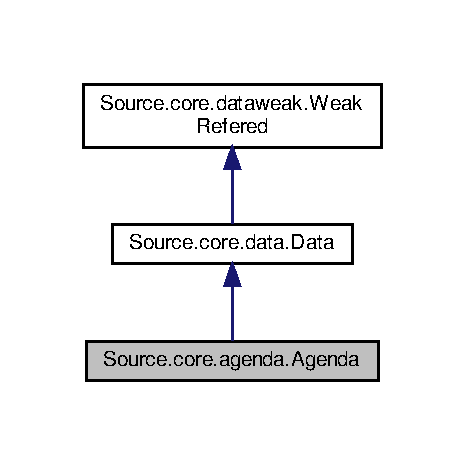
\includegraphics[width=223pt]{classSource_1_1core_1_1agenda_1_1Agenda__inherit__graph}
\end{center}
\end{figure}


Collaboration diagram for Source.\+core.\+agenda.\+Agenda\+:\nopagebreak
\begin{figure}[H]
\begin{center}
\leavevmode
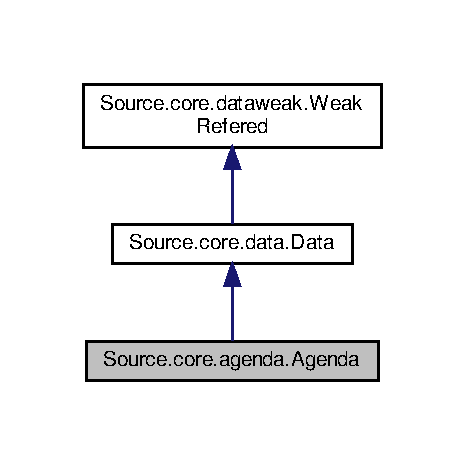
\includegraphics[width=223pt]{classSource_1_1core_1_1agenda_1_1Agenda__coll__graph}
\end{center}
\end{figure}
\subsection*{Public Member Functions}
\begin{DoxyCompactItemize}
\item 
def \mbox{\hyperlink{classSource_1_1core_1_1agenda_1_1Agenda_a38a1269669d7526f710087a278d70c39}{\+\_\+\+\_\+init\+\_\+\+\_\+}} (self, \+\_\+id, collection, name, linked\+\_\+agendas, notifications, ignored\+\_\+events, last\+\_\+sync=None, user=None, group=None)
\begin{DoxyCompactList}\small\item\em Création d\textquotesingle{}un agenda. \end{DoxyCompactList}\item 
\mbox{\Hypertarget{classSource_1_1core_1_1agenda_1_1Agenda_a3913a072c5efcc3a84111d48ea0b34cc}\label{classSource_1_1core_1_1agenda_1_1Agenda_a3913a072c5efcc3a84111d48ea0b34cc}} 
def \mbox{\hyperlink{classSource_1_1core_1_1agenda_1_1Agenda_a3913a072c5efcc3a84111d48ea0b34cc}{\+\_\+\+\_\+repr\+\_\+\+\_\+}} (self)
\begin{DoxyCompactList}\small\item\em affiche l\textquotesingle{}agenda \end{DoxyCompactList}\item 
def \mbox{\hyperlink{classSource_1_1core_1_1agenda_1_1Agenda_af0e83535fec55d0cd9d15e24db3ae4a5}{add\+\_\+event}} (self, event)
\begin{DoxyCompactList}\small\item\em Ajout d\textquotesingle{}un evenement. \end{DoxyCompactList}\item 
def \mbox{\hyperlink{classSource_1_1core_1_1agenda_1_1Agenda_a2a56040b52078f048e1ce04a647b3ad5}{remove\+\_\+event}} (self, event)
\begin{DoxyCompactList}\small\item\em Suppression d\textquotesingle{}un evenement. \end{DoxyCompactList}\item 
\mbox{\Hypertarget{classSource_1_1core_1_1agenda_1_1Agenda_ab1529afbf0b57577dade2cc216bdcaaa}\label{classSource_1_1core_1_1agenda_1_1Agenda_ab1529afbf0b57577dade2cc216bdcaaa}} 
def \mbox{\hyperlink{classSource_1_1core_1_1agenda_1_1Agenda_ab1529afbf0b57577dade2cc216bdcaaa}{events}} (self, from\+\_\+date, to\+\_\+date)
\begin{DoxyCompactList}\small\item\em Obtention des événements propre à l\textquotesingle{}agenda sur une période. \end{DoxyCompactList}\item 
\mbox{\Hypertarget{classSource_1_1core_1_1agenda_1_1Agenda_ad00ef12f8cab0332d96234f094b66e6b}\label{classSource_1_1core_1_1agenda_1_1Agenda_ad00ef12f8cab0332d96234f094b66e6b}} 
def \mbox{\hyperlink{classSource_1_1core_1_1agenda_1_1Agenda_ad00ef12f8cab0332d96234f094b66e6b}{all\+\_\+events}} (self, from\+\_\+date, to\+\_\+date)
\begin{DoxyCompactList}\small\item\em Renvoi tous les évenement avec ceux des agendas liés. \end{DoxyCompactList}\item 
\mbox{\Hypertarget{classSource_1_1core_1_1agenda_1_1Agenda_a92e46c6575dcbb5c6ae030e4420d7030}\label{classSource_1_1core_1_1agenda_1_1Agenda_a92e46c6575dcbb5c6ae030e4420d7030}} 
def \mbox{\hyperlink{classSource_1_1core_1_1agenda_1_1Agenda_a92e46c6575dcbb5c6ae030e4420d7030}{last\+\_\+events}} (self, last\+\_\+date)
\begin{DoxyCompactList}\small\item\em Chargement de plus d\textquotesingle{}événements récent. \end{DoxyCompactList}\item 
def \mbox{\hyperlink{classSource_1_1core_1_1agenda_1_1Agenda_a49963bf70decca8bf319f4487ff90e47}{sync\+\_\+notifications}} (self)
\begin{DoxyCompactList}\small\item\em Créer des notifications pour les nouveau événements extérieurs. \end{DoxyCompactList}\item 
def \mbox{\hyperlink{classSource_1_1core_1_1agenda_1_1Agenda_a40d2789a7f02d15bfd205c1be9b82814}{add\+\_\+notification}} (self, notification)
\begin{DoxyCompactList}\small\item\em Ajout d\textquotesingle{}une notification de cet agenda. \end{DoxyCompactList}\item 
def \mbox{\hyperlink{classSource_1_1core_1_1agenda_1_1Agenda_a34ea6d5e23cfc5aeb271ba1d2b1eb9c4}{remove\+\_\+notification}} (self, notification, ignore)
\begin{DoxyCompactList}\small\item\em Suppression d\textquotesingle{}une notification de cet agenda. \end{DoxyCompactList}\item 
def \mbox{\hyperlink{classSource_1_1core_1_1agenda_1_1Agenda_a8507315e466edecb3c514524e0921050}{link\+\_\+agenda}} (self, agenda)
\begin{DoxyCompactList}\small\item\em Ajout d\textquotesingle{}un lien vers un autre agenda. \end{DoxyCompactList}\item 
def \mbox{\hyperlink{classSource_1_1core_1_1agenda_1_1Agenda_a5fc4d8bb32863edde30afa3474da14c2}{unlink\+\_\+agenda}} (self, agenda)
\begin{DoxyCompactList}\small\item\em Suppression d\textquotesingle{}un lien vers un autre agenda. \end{DoxyCompactList}\end{DoxyCompactItemize}
\subsection*{Public Attributes}
\begin{DoxyCompactItemize}
\item 
\mbox{\Hypertarget{classSource_1_1core_1_1agenda_1_1Agenda_a030252a43b5bb8b7831f99b288c2bbed}\label{classSource_1_1core_1_1agenda_1_1Agenda_a030252a43b5bb8b7831f99b288c2bbed}} 
{\bfseries linked\+\_\+agendas}
\item 
\mbox{\Hypertarget{classSource_1_1core_1_1agenda_1_1Agenda_a92b05868c7dbbda031b212d934c03063}\label{classSource_1_1core_1_1agenda_1_1Agenda_a92b05868c7dbbda031b212d934c03063}} 
{\bfseries notifications}
\item 
\mbox{\Hypertarget{classSource_1_1core_1_1agenda_1_1Agenda_a59000cbbdda47730a18a017b5605d88a}\label{classSource_1_1core_1_1agenda_1_1Agenda_a59000cbbdda47730a18a017b5605d88a}} 
{\bfseries ignored\+\_\+events}
\end{DoxyCompactItemize}
\subsection*{Static Public Attributes}
\begin{DoxyCompactItemize}
\item 
\mbox{\Hypertarget{classSource_1_1core_1_1agenda_1_1Agenda_a1fd989185247a660202ad85467fa9e09}\label{classSource_1_1core_1_1agenda_1_1Agenda_a1fd989185247a660202ad85467fa9e09}} 
{\bfseries name} = \mbox{\hyperlink{classSource_1_1core_1_1dataproperty_1_1DataProperty}{Data\+Property}}(\char`\"{}name\char`\"{})
\item 
\mbox{\Hypertarget{classSource_1_1core_1_1agenda_1_1Agenda_ace3b88d98bdde2583c87eec36f000643}\label{classSource_1_1core_1_1agenda_1_1Agenda_ace3b88d98bdde2583c87eec36f000643}} 
{\bfseries last\+\_\+sync} = \mbox{\hyperlink{classSource_1_1core_1_1dataproperty_1_1DataProperty}{Data\+Property}}(\char`\"{}last\+\_\+sync\char`\"{})
\item 
\mbox{\Hypertarget{classSource_1_1core_1_1agenda_1_1Agenda_a94ba7fe2ea0846fd3c4f8589a8789f7b}\label{classSource_1_1core_1_1agenda_1_1Agenda_a94ba7fe2ea0846fd3c4f8589a8789f7b}} 
{\bfseries user} = \mbox{\hyperlink{classSource_1_1core_1_1dataproperty_1_1DataOwnerProperty}{Data\+Owner\+Property}}(\char`\"{}user\char`\"{})
\item 
\mbox{\Hypertarget{classSource_1_1core_1_1agenda_1_1Agenda_a66df05ea797e5d88342a67905a1c7fd7}\label{classSource_1_1core_1_1agenda_1_1Agenda_a66df05ea797e5d88342a67905a1c7fd7}} 
{\bfseries group} = \mbox{\hyperlink{classSource_1_1core_1_1dataproperty_1_1DataOwnerProperty}{Data\+Owner\+Property}}(\char`\"{}group\char`\"{})
\end{DoxyCompactItemize}


\subsection{Constructor \& Destructor Documentation}
\mbox{\Hypertarget{classSource_1_1core_1_1agenda_1_1Agenda_a38a1269669d7526f710087a278d70c39}\label{classSource_1_1core_1_1agenda_1_1Agenda_a38a1269669d7526f710087a278d70c39}} 
\index{Source\+::core\+::agenda\+::\+Agenda@{Source\+::core\+::agenda\+::\+Agenda}!\+\_\+\+\_\+init\+\_\+\+\_\+@{\+\_\+\+\_\+init\+\_\+\+\_\+}}
\index{\+\_\+\+\_\+init\+\_\+\+\_\+@{\+\_\+\+\_\+init\+\_\+\+\_\+}!Source\+::core\+::agenda\+::\+Agenda@{Source\+::core\+::agenda\+::\+Agenda}}
\subsubsection{\texorpdfstring{\+\_\+\+\_\+init\+\_\+\+\_\+()}{\_\_init\_\_()}}
{\footnotesize\ttfamily def Source.\+core.\+agenda.\+Agenda.\+\_\+\+\_\+init\+\_\+\+\_\+ (\begin{DoxyParamCaption}\item[{}]{self,  }\item[{}]{\+\_\+id,  }\item[{}]{collection,  }\item[{}]{name,  }\item[{}]{linked\+\_\+agendas,  }\item[{}]{notifications,  }\item[{}]{ignored\+\_\+events,  }\item[{}]{last\+\_\+sync = {\ttfamily None},  }\item[{}]{user = {\ttfamily None},  }\item[{}]{group = {\ttfamily None} }\end{DoxyParamCaption})}



Création d\textquotesingle{}un agenda. 


\begin{DoxyParams}{Parameters}
{\em collection} & \+: la collection a passer (dans le fichier common). \\
\hline
{\em name} & \+: nom de l\textquotesingle{}agenda \\
\hline
{\em linked\+\_\+agendas} & \+: liste des agendas associés à l\textquotesingle{}agenda \\
\hline
{\em notifications} & \+: liste des notifications liés à l\textquotesingle{}agenda. \\
\hline
{\em ignored\+\_\+events} & \+: les évènements ni en attentes ? \\
\hline
\end{DoxyParams}


\subsection{Member Function Documentation}
\mbox{\Hypertarget{classSource_1_1core_1_1agenda_1_1Agenda_af0e83535fec55d0cd9d15e24db3ae4a5}\label{classSource_1_1core_1_1agenda_1_1Agenda_af0e83535fec55d0cd9d15e24db3ae4a5}} 
\index{Source\+::core\+::agenda\+::\+Agenda@{Source\+::core\+::agenda\+::\+Agenda}!add\+\_\+event@{add\+\_\+event}}
\index{add\+\_\+event@{add\+\_\+event}!Source\+::core\+::agenda\+::\+Agenda@{Source\+::core\+::agenda\+::\+Agenda}}
\subsubsection{\texorpdfstring{add\+\_\+event()}{add\_event()}}
{\footnotesize\ttfamily def Source.\+core.\+agenda.\+Agenda.\+add\+\_\+event (\begin{DoxyParamCaption}\item[{}]{self,  }\item[{}]{event }\end{DoxyParamCaption})}



Ajout d\textquotesingle{}un evenement. 

Here is the call graph for this function\+:
\nopagebreak
\begin{figure}[H]
\begin{center}
\leavevmode
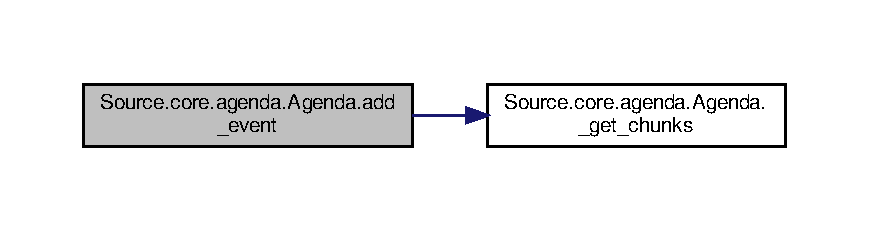
\includegraphics[width=350pt]{classSource_1_1core_1_1agenda_1_1Agenda_af0e83535fec55d0cd9d15e24db3ae4a5_cgraph}
\end{center}
\end{figure}
\mbox{\Hypertarget{classSource_1_1core_1_1agenda_1_1Agenda_a40d2789a7f02d15bfd205c1be9b82814}\label{classSource_1_1core_1_1agenda_1_1Agenda_a40d2789a7f02d15bfd205c1be9b82814}} 
\index{Source\+::core\+::agenda\+::\+Agenda@{Source\+::core\+::agenda\+::\+Agenda}!add\+\_\+notification@{add\+\_\+notification}}
\index{add\+\_\+notification@{add\+\_\+notification}!Source\+::core\+::agenda\+::\+Agenda@{Source\+::core\+::agenda\+::\+Agenda}}
\subsubsection{\texorpdfstring{add\+\_\+notification()}{add\_notification()}}
{\footnotesize\ttfamily def Source.\+core.\+agenda.\+Agenda.\+add\+\_\+notification (\begin{DoxyParamCaption}\item[{}]{self,  }\item[{}]{notification }\end{DoxyParamCaption})}



Ajout d\textquotesingle{}une notification de cet agenda. 

\mbox{\Hypertarget{classSource_1_1core_1_1agenda_1_1Agenda_a8507315e466edecb3c514524e0921050}\label{classSource_1_1core_1_1agenda_1_1Agenda_a8507315e466edecb3c514524e0921050}} 
\index{Source\+::core\+::agenda\+::\+Agenda@{Source\+::core\+::agenda\+::\+Agenda}!link\+\_\+agenda@{link\+\_\+agenda}}
\index{link\+\_\+agenda@{link\+\_\+agenda}!Source\+::core\+::agenda\+::\+Agenda@{Source\+::core\+::agenda\+::\+Agenda}}
\subsubsection{\texorpdfstring{link\+\_\+agenda()}{link\_agenda()}}
{\footnotesize\ttfamily def Source.\+core.\+agenda.\+Agenda.\+link\+\_\+agenda (\begin{DoxyParamCaption}\item[{}]{self,  }\item[{}]{agenda }\end{DoxyParamCaption})}



Ajout d\textquotesingle{}un lien vers un autre agenda. 

\mbox{\Hypertarget{classSource_1_1core_1_1agenda_1_1Agenda_a2a56040b52078f048e1ce04a647b3ad5}\label{classSource_1_1core_1_1agenda_1_1Agenda_a2a56040b52078f048e1ce04a647b3ad5}} 
\index{Source\+::core\+::agenda\+::\+Agenda@{Source\+::core\+::agenda\+::\+Agenda}!remove\+\_\+event@{remove\+\_\+event}}
\index{remove\+\_\+event@{remove\+\_\+event}!Source\+::core\+::agenda\+::\+Agenda@{Source\+::core\+::agenda\+::\+Agenda}}
\subsubsection{\texorpdfstring{remove\+\_\+event()}{remove\_event()}}
{\footnotesize\ttfamily def Source.\+core.\+agenda.\+Agenda.\+remove\+\_\+event (\begin{DoxyParamCaption}\item[{}]{self,  }\item[{}]{event }\end{DoxyParamCaption})}



Suppression d\textquotesingle{}un evenement. 

Here is the call graph for this function\+:
\nopagebreak
\begin{figure}[H]
\begin{center}
\leavevmode
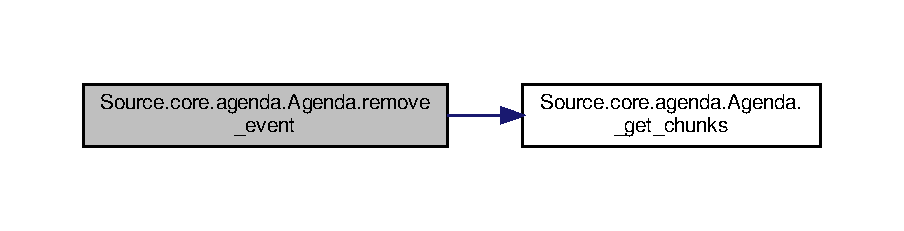
\includegraphics[width=350pt]{classSource_1_1core_1_1agenda_1_1Agenda_a2a56040b52078f048e1ce04a647b3ad5_cgraph}
\end{center}
\end{figure}
\mbox{\Hypertarget{classSource_1_1core_1_1agenda_1_1Agenda_a34ea6d5e23cfc5aeb271ba1d2b1eb9c4}\label{classSource_1_1core_1_1agenda_1_1Agenda_a34ea6d5e23cfc5aeb271ba1d2b1eb9c4}} 
\index{Source\+::core\+::agenda\+::\+Agenda@{Source\+::core\+::agenda\+::\+Agenda}!remove\+\_\+notification@{remove\+\_\+notification}}
\index{remove\+\_\+notification@{remove\+\_\+notification}!Source\+::core\+::agenda\+::\+Agenda@{Source\+::core\+::agenda\+::\+Agenda}}
\subsubsection{\texorpdfstring{remove\+\_\+notification()}{remove\_notification()}}
{\footnotesize\ttfamily def Source.\+core.\+agenda.\+Agenda.\+remove\+\_\+notification (\begin{DoxyParamCaption}\item[{}]{self,  }\item[{}]{notification,  }\item[{}]{ignore }\end{DoxyParamCaption})}



Suppression d\textquotesingle{}une notification de cet agenda. 

\mbox{\Hypertarget{classSource_1_1core_1_1agenda_1_1Agenda_a49963bf70decca8bf319f4487ff90e47}\label{classSource_1_1core_1_1agenda_1_1Agenda_a49963bf70decca8bf319f4487ff90e47}} 
\index{Source\+::core\+::agenda\+::\+Agenda@{Source\+::core\+::agenda\+::\+Agenda}!sync\+\_\+notifications@{sync\+\_\+notifications}}
\index{sync\+\_\+notifications@{sync\+\_\+notifications}!Source\+::core\+::agenda\+::\+Agenda@{Source\+::core\+::agenda\+::\+Agenda}}
\subsubsection{\texorpdfstring{sync\+\_\+notifications()}{sync\_notifications()}}
{\footnotesize\ttfamily def Source.\+core.\+agenda.\+Agenda.\+sync\+\_\+notifications (\begin{DoxyParamCaption}\item[{}]{self }\end{DoxyParamCaption})}



Créer des notifications pour les nouveau événements extérieurs. 

\mbox{\Hypertarget{classSource_1_1core_1_1agenda_1_1Agenda_a5fc4d8bb32863edde30afa3474da14c2}\label{classSource_1_1core_1_1agenda_1_1Agenda_a5fc4d8bb32863edde30afa3474da14c2}} 
\index{Source\+::core\+::agenda\+::\+Agenda@{Source\+::core\+::agenda\+::\+Agenda}!unlink\+\_\+agenda@{unlink\+\_\+agenda}}
\index{unlink\+\_\+agenda@{unlink\+\_\+agenda}!Source\+::core\+::agenda\+::\+Agenda@{Source\+::core\+::agenda\+::\+Agenda}}
\subsubsection{\texorpdfstring{unlink\+\_\+agenda()}{unlink\_agenda()}}
{\footnotesize\ttfamily def Source.\+core.\+agenda.\+Agenda.\+unlink\+\_\+agenda (\begin{DoxyParamCaption}\item[{}]{self,  }\item[{}]{agenda }\end{DoxyParamCaption})}



Suppression d\textquotesingle{}un lien vers un autre agenda. 



The documentation for this class was generated from the following file\+:\begin{DoxyCompactItemize}
\item 
/home/tristan/\+Documents/\+U\+S\+M\+B/\+I\+N\+F\+O\+\_\+406/\+Source/core/agenda.\+py\end{DoxyCompactItemize}

\hypertarget{classSource_1_1core_1_1collection_1_1Collection}{}\section{Source.\+core.\+collection.\+Collection Class Reference}
\label{classSource_1_1core_1_1collection_1_1Collection}\index{Source.\+core.\+collection.\+Collection@{Source.\+core.\+collection.\+Collection}}


\mbox{\hyperlink{classSource_1_1core_1_1collection_1_1Collection}{Collection}} de toutes les données du système.  


\subsection*{Public Member Functions}
\begin{DoxyCompactItemize}
\item 
def \mbox{\hyperlink{classSource_1_1core_1_1collection_1_1Collection_a916198d63b982729e8fd286414436392}{load}} (self, \+\_\+id, type)
\begin{DoxyCompactList}\small\item\em Charge une données selon son type et id. \end{DoxyCompactList}\item 
\mbox{\Hypertarget{classSource_1_1core_1_1collection_1_1Collection_ae81f49621b4c1fbaa341cbef7c95d7b7}\label{classSource_1_1core_1_1collection_1_1Collection_ae81f49621b4c1fbaa341cbef7c95d7b7}} 
def {\bfseries load\+\_\+events} (self, agenda, month\+\_\+first\+\_\+day, next\+\_\+month\+\_\+first\+\_\+day)
\item 
\mbox{\Hypertarget{classSource_1_1core_1_1collection_1_1Collection_aef2f107a35b1a896a196772fc0d4cc7b}\label{classSource_1_1core_1_1collection_1_1Collection_aef2f107a35b1a896a196772fc0d4cc7b}} 
def {\bfseries load\+\_\+latest\+\_\+events} (self, agenda, last\+\_\+sync)
\item 
\mbox{\Hypertarget{classSource_1_1core_1_1collection_1_1Collection_a42cd0fa5c539ebde2ca6c1449daa5e36}\label{classSource_1_1core_1_1collection_1_1Collection_a42cd0fa5c539ebde2ca6c1449daa5e36}} 
def {\bfseries new} (self, type, args)
\item 
\mbox{\Hypertarget{classSource_1_1core_1_1collection_1_1Collection_a3975c671f12597b018d0b9a036c43508}\label{classSource_1_1core_1_1collection_1_1Collection_a3975c671f12597b018d0b9a036c43508}} 
def {\bfseries delete} (self, data)
\item 
\mbox{\Hypertarget{classSource_1_1core_1_1collection_1_1Collection_ae3005c8d2ffe8eeeceef8876ba2ba436}\label{classSource_1_1core_1_1collection_1_1Collection_ae3005c8d2ffe8eeeceef8876ba2ba436}} 
def {\bfseries delete\+\_\+proxy} (self, proxy)
\item 
\mbox{\Hypertarget{classSource_1_1core_1_1collection_1_1Collection_a2b16760f8357a116183e41b4aaa27881}\label{classSource_1_1core_1_1collection_1_1Collection_a2b16760f8357a116183e41b4aaa27881}} 
def {\bfseries update} (self, data)
\item 
\mbox{\Hypertarget{classSource_1_1core_1_1collection_1_1Collection_a113774e3faf43823fd27a40b2435c276}\label{classSource_1_1core_1_1collection_1_1Collection_a113774e3faf43823fd27a40b2435c276}} 
def {\bfseries update\+\_\+relations} (self, data)
\end{DoxyCompactItemize}


\subsection{Detailed Description}
\mbox{\hyperlink{classSource_1_1core_1_1collection_1_1Collection}{Collection}} de toutes les données du système. 

À chaque accès à un data proxy n\textquotesingle{}ayant pas chargé sa data la collection est appellé pour la charger.

Ceci est possible depuis une B\+DD ou par réseau, d\textquotesingle{}où deux classes filles de la classe \mbox{\hyperlink{classSource_1_1core_1_1collection_1_1Collection}{Collection}}. 

\subsection{Member Function Documentation}
\mbox{\Hypertarget{classSource_1_1core_1_1collection_1_1Collection_a916198d63b982729e8fd286414436392}\label{classSource_1_1core_1_1collection_1_1Collection_a916198d63b982729e8fd286414436392}} 
\index{Source\+::core\+::collection\+::\+Collection@{Source\+::core\+::collection\+::\+Collection}!load@{load}}
\index{load@{load}!Source\+::core\+::collection\+::\+Collection@{Source\+::core\+::collection\+::\+Collection}}
\subsubsection{\texorpdfstring{load()}{load()}}
{\footnotesize\ttfamily def Source.\+core.\+collection.\+Collection.\+load (\begin{DoxyParamCaption}\item[{}]{self,  }\item[{}]{\+\_\+id,  }\item[{}]{type }\end{DoxyParamCaption})}



Charge une données selon son type et id. 



The documentation for this class was generated from the following file\+:\begin{DoxyCompactItemize}
\item 
/home/tristan/\+Documents/\+U\+S\+M\+B/\+I\+N\+F\+O\+\_\+406/\+Source/core/collection.\+py\end{DoxyCompactItemize}

\hypertarget{classSource_1_1core_1_1data_1_1Data}{}\section{Source.\+core.\+data.\+Data Class Reference}
\label{classSource_1_1core_1_1data_1_1Data}\index{Source.\+core.\+data.\+Data@{Source.\+core.\+data.\+Data}}


Inheritance diagram for Source.\+core.\+data.\+Data\+:\nopagebreak
\begin{figure}[H]
\begin{center}
\leavevmode
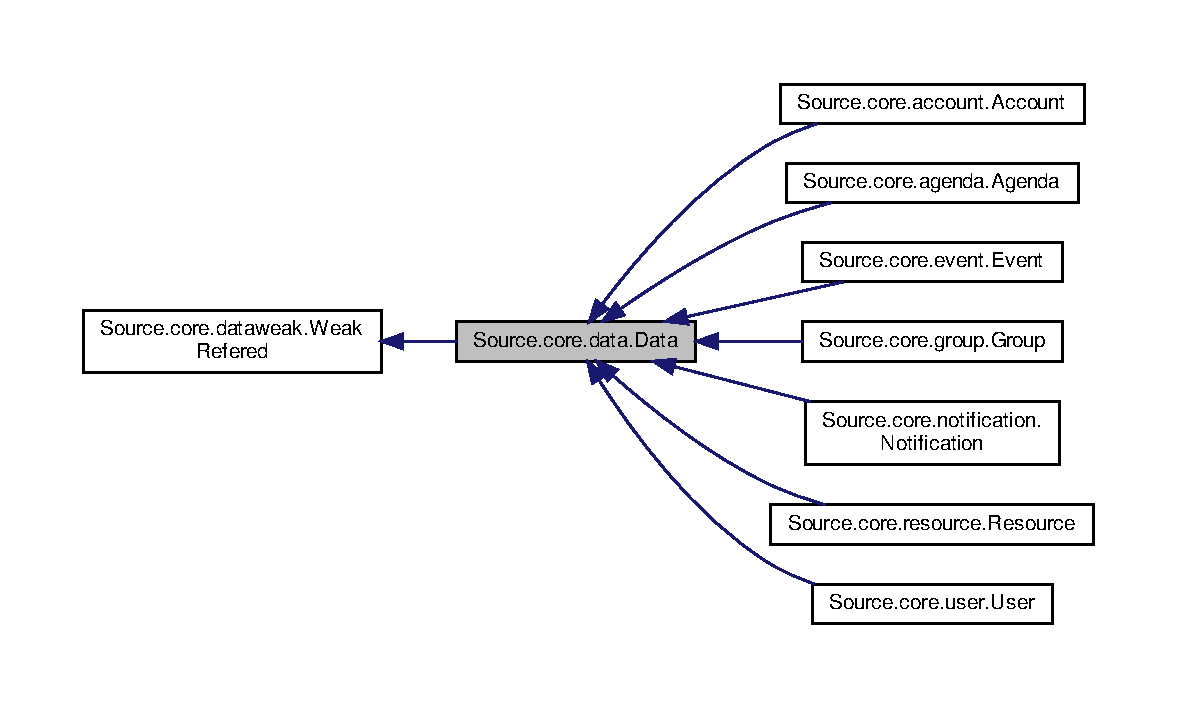
\includegraphics[width=350pt]{classSource_1_1core_1_1data_1_1Data__inherit__graph}
\end{center}
\end{figure}


Collaboration diagram for Source.\+core.\+data.\+Data\+:\nopagebreak
\begin{figure}[H]
\begin{center}
\leavevmode
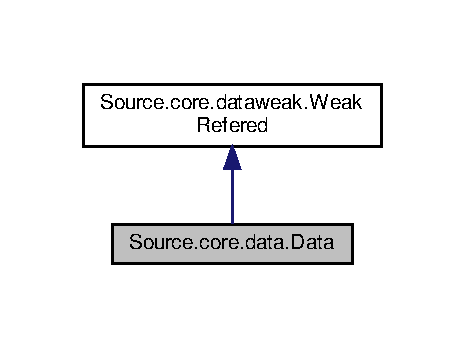
\includegraphics[width=223pt]{classSource_1_1core_1_1data_1_1Data__coll__graph}
\end{center}
\end{figure}
\subsection*{Public Member Functions}
\begin{DoxyCompactItemize}
\item 
\mbox{\Hypertarget{classSource_1_1core_1_1data_1_1Data_aabb409fc5f61a6cc4958785d97ead581}\label{classSource_1_1core_1_1data_1_1Data_aabb409fc5f61a6cc4958785d97ead581}} 
def {\bfseries \+\_\+\+\_\+init\+\_\+\+\_\+} (self, \+\_\+id, collection)
\item 
\mbox{\Hypertarget{classSource_1_1core_1_1data_1_1Data_a238106c23f9485029a6b7a5468f55045}\label{classSource_1_1core_1_1data_1_1Data_a238106c23f9485029a6b7a5468f55045}} 
def {\bfseries new} (cls, collection, args)
\item 
\mbox{\Hypertarget{classSource_1_1core_1_1data_1_1Data_a33f5cd6a28cc05f318226d7212fd8c2e}\label{classSource_1_1core_1_1data_1_1Data_a33f5cd6a28cc05f318226d7212fd8c2e}} 
def {\bfseries load} (cls, collection, \+\_\+id)
\item 
\mbox{\Hypertarget{classSource_1_1core_1_1data_1_1Data_a12c16d466abfbf9974f6357fc805a0f5}\label{classSource_1_1core_1_1data_1_1Data_a12c16d466abfbf9974f6357fc805a0f5}} 
def {\bfseries delete} (self, owner=None)
\item 
\mbox{\Hypertarget{classSource_1_1core_1_1data_1_1Data_a6630f7e7d66c3b7966a78c727acb9368}\label{classSource_1_1core_1_1data_1_1Data_a6630f7e7d66c3b7966a78c727acb9368}} 
def {\bfseries update} (self)
\item 
def \mbox{\hyperlink{classSource_1_1core_1_1data_1_1Data_a234b982c5580ac03d31f4e8db8ee87a5}{update\+\_\+relations}} (self)
\begin{DoxyCompactList}\small\item\em Actualisation des relations seulements. \end{DoxyCompactList}\item 
\mbox{\Hypertarget{classSource_1_1core_1_1data_1_1Data_adf7a236f85f581437fc62a8319b6d083}\label{classSource_1_1core_1_1data_1_1Data_adf7a236f85f581437fc62a8319b6d083}} 
def {\bfseries \+\_\+\+\_\+hash\+\_\+\+\_\+} (self)
\item 
\mbox{\Hypertarget{classSource_1_1core_1_1data_1_1Data_a3616f6e7c12a6463757879c9263fddbd}\label{classSource_1_1core_1_1data_1_1Data_a3616f6e7c12a6463757879c9263fddbd}} 
def {\bfseries \+\_\+\+\_\+eq\+\_\+\+\_\+} (self, other)
\end{DoxyCompactItemize}
\subsection*{Public Attributes}
\begin{DoxyCompactItemize}
\item 
\mbox{\Hypertarget{classSource_1_1core_1_1data_1_1Data_a8cb11df2a94acd2b3c77eb606e80775d}\label{classSource_1_1core_1_1data_1_1Data_a8cb11df2a94acd2b3c77eb606e80775d}} 
{\bfseries id}
\item 
\mbox{\Hypertarget{classSource_1_1core_1_1data_1_1Data_a0a9994330613d8f2fceda8175abcd2ce}\label{classSource_1_1core_1_1data_1_1Data_a0a9994330613d8f2fceda8175abcd2ce}} 
{\bfseries collection}
\item 
\mbox{\Hypertarget{classSource_1_1core_1_1data_1_1Data_a2d7bdfd4790514816bffe31175e132f3}\label{classSource_1_1core_1_1data_1_1Data_a2d7bdfd4790514816bffe31175e132f3}} 
{\bfseries proxy}
\end{DoxyCompactItemize}


\subsection{Member Function Documentation}
\mbox{\Hypertarget{classSource_1_1core_1_1data_1_1Data_a234b982c5580ac03d31f4e8db8ee87a5}\label{classSource_1_1core_1_1data_1_1Data_a234b982c5580ac03d31f4e8db8ee87a5}} 
\index{Source\+::core\+::data\+::\+Data@{Source\+::core\+::data\+::\+Data}!update\+\_\+relations@{update\+\_\+relations}}
\index{update\+\_\+relations@{update\+\_\+relations}!Source\+::core\+::data\+::\+Data@{Source\+::core\+::data\+::\+Data}}
\subsubsection{\texorpdfstring{update\+\_\+relations()}{update\_relations()}}
{\footnotesize\ttfamily def Source.\+core.\+data.\+Data.\+update\+\_\+relations (\begin{DoxyParamCaption}\item[{}]{self }\end{DoxyParamCaption})}



Actualisation des relations seulements. 

Par exemple lors d\textquotesingle{}ajout d\textquotesingle{}un utilisateur dans un groupe, d\textquotesingle{}un administrateur. 

The documentation for this class was generated from the following file\+:\begin{DoxyCompactItemize}
\item 
/home/tristan/\+Documents/\+U\+S\+M\+B/\+I\+N\+F\+O\+\_\+406/\+Source/core/data.\+py\end{DoxyCompactItemize}

\hypertarget{classSource_1_1core_1_1dataproperty_1_1DataOwnerProperty}{}\section{Source.\+core.\+dataproperty.\+Data\+Owner\+Property Class Reference}
\label{classSource_1_1core_1_1dataproperty_1_1DataOwnerProperty}\index{Source.\+core.\+dataproperty.\+Data\+Owner\+Property@{Source.\+core.\+dataproperty.\+Data\+Owner\+Property}}


Inheritance diagram for Source.\+core.\+dataproperty.\+Data\+Owner\+Property\+:\nopagebreak
\begin{figure}[H]
\begin{center}
\leavevmode
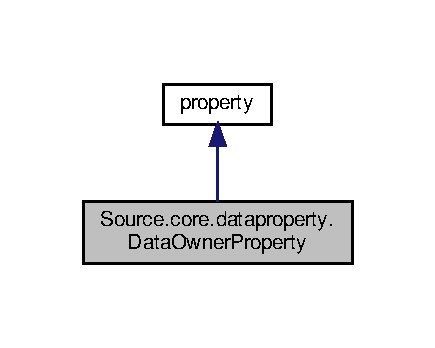
\includegraphics[width=209pt]{classSource_1_1core_1_1dataproperty_1_1DataOwnerProperty__inherit__graph}
\end{center}
\end{figure}


Collaboration diagram for Source.\+core.\+dataproperty.\+Data\+Owner\+Property\+:\nopagebreak
\begin{figure}[H]
\begin{center}
\leavevmode
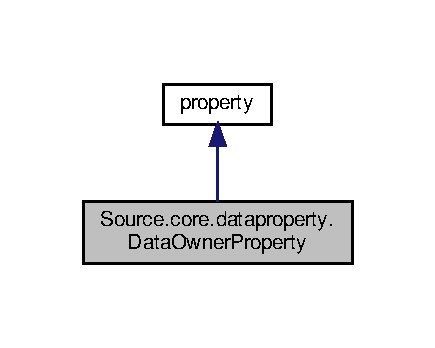
\includegraphics[width=209pt]{classSource_1_1core_1_1dataproperty_1_1DataOwnerProperty__coll__graph}
\end{center}
\end{figure}
\subsection*{Public Member Functions}
\begin{DoxyCompactItemize}
\item 
\mbox{\Hypertarget{classSource_1_1core_1_1dataproperty_1_1DataOwnerProperty_a42524065b086a21700354af955337fe5}\label{classSource_1_1core_1_1dataproperty_1_1DataOwnerProperty_a42524065b086a21700354af955337fe5}} 
def {\bfseries \+\_\+\+\_\+init\+\_\+\+\_\+} (self, attr\+\_\+name)
\end{DoxyCompactItemize}
\subsection*{Static Public Member Functions}
\begin{DoxyCompactItemize}
\item 
\mbox{\Hypertarget{classSource_1_1core_1_1dataproperty_1_1DataOwnerProperty_a30a34a0351b370b8377b1ba028d47c15}\label{classSource_1_1core_1_1dataproperty_1_1DataOwnerProperty_a30a34a0351b370b8377b1ba028d47c15}} 
def \mbox{\hyperlink{classSource_1_1core_1_1dataproperty_1_1DataOwnerProperty_a30a34a0351b370b8377b1ba028d47c15}{init}} (reffered, refferer)
\begin{DoxyCompactList}\small\item\em Initialise une référence faible Utilisé dans le constructeur sans passer par le setter de \mbox{\hyperlink{classSource_1_1core_1_1dataproperty_1_1DataOwnerProperty}{Data\+Owner\+Property}} qui va appeller update() \end{DoxyCompactList}\end{DoxyCompactItemize}


The documentation for this class was generated from the following file\+:\begin{DoxyCompactItemize}
\item 
/home/tristan/\+Documents/\+U\+S\+M\+B/\+I\+N\+F\+O\+\_\+406/\+Source/core/dataproperty.\+py\end{DoxyCompactItemize}

\hypertarget{classSource_1_1core_1_1dataproperty_1_1DataProperty}{}\section{Source.\+core.\+dataproperty.\+Data\+Property Class Reference}
\label{classSource_1_1core_1_1dataproperty_1_1DataProperty}\index{Source.\+core.\+dataproperty.\+Data\+Property@{Source.\+core.\+dataproperty.\+Data\+Property}}


Inheritance diagram for Source.\+core.\+dataproperty.\+Data\+Property\+:\nopagebreak
\begin{figure}[H]
\begin{center}
\leavevmode
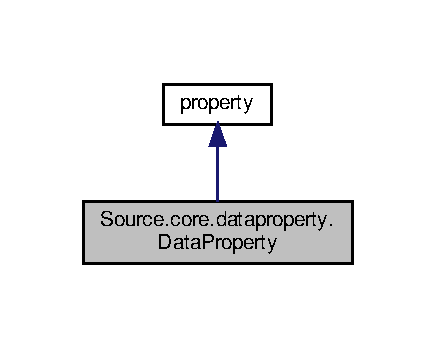
\includegraphics[width=209pt]{classSource_1_1core_1_1dataproperty_1_1DataProperty__inherit__graph}
\end{center}
\end{figure}


Collaboration diagram for Source.\+core.\+dataproperty.\+Data\+Property\+:\nopagebreak
\begin{figure}[H]
\begin{center}
\leavevmode
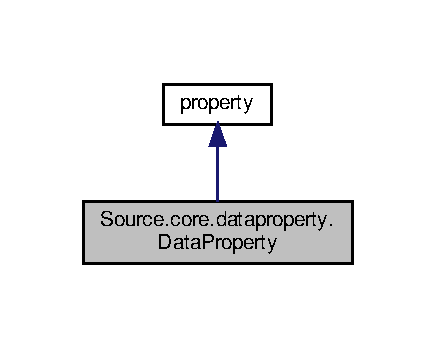
\includegraphics[width=209pt]{classSource_1_1core_1_1dataproperty_1_1DataProperty__coll__graph}
\end{center}
\end{figure}
\subsection*{Public Member Functions}
\begin{DoxyCompactItemize}
\item 
\mbox{\Hypertarget{classSource_1_1core_1_1dataproperty_1_1DataProperty_ad12c5230c3e926e3232ea586a99625e4}\label{classSource_1_1core_1_1dataproperty_1_1DataProperty_ad12c5230c3e926e3232ea586a99625e4}} 
def {\bfseries \+\_\+\+\_\+init\+\_\+\+\_\+} (self, attr\+\_\+name)
\end{DoxyCompactItemize}


The documentation for this class was generated from the following file\+:\begin{DoxyCompactItemize}
\item 
/home/tristan/\+Documents/\+U\+S\+M\+B/\+I\+N\+F\+O\+\_\+406/\+Source/core/dataproperty.\+py\end{DoxyCompactItemize}

\hypertarget{classSource_1_1core_1_1dataproxy_1_1DataProxy}{}\section{Source.\+core.\+dataproxy.\+Data\+Proxy Class Reference}
\label{classSource_1_1core_1_1dataproxy_1_1DataProxy}\index{Source.\+core.\+dataproxy.\+Data\+Proxy@{Source.\+core.\+dataproxy.\+Data\+Proxy}}


Inheritance diagram for Source.\+core.\+dataproxy.\+Data\+Proxy\+:\nopagebreak
\begin{figure}[H]
\begin{center}
\leavevmode
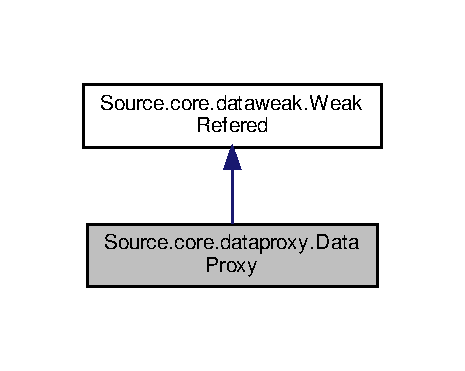
\includegraphics[width=223pt]{classSource_1_1core_1_1dataproxy_1_1DataProxy__inherit__graph}
\end{center}
\end{figure}


Collaboration diagram for Source.\+core.\+dataproxy.\+Data\+Proxy\+:\nopagebreak
\begin{figure}[H]
\begin{center}
\leavevmode
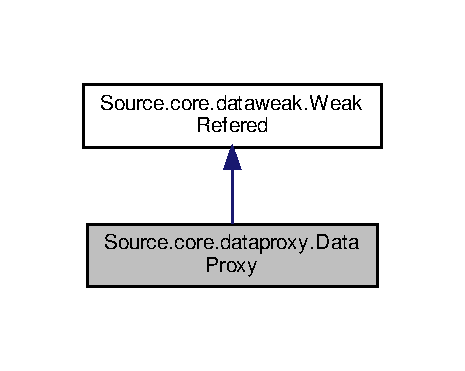
\includegraphics[width=223pt]{classSource_1_1core_1_1dataproxy_1_1DataProxy__coll__graph}
\end{center}
\end{figure}
\subsection*{Public Member Functions}
\begin{DoxyCompactItemize}
\item 
\mbox{\Hypertarget{classSource_1_1core_1_1dataproxy_1_1DataProxy_a17a6e79d81a281493af68e92ff537ec5}\label{classSource_1_1core_1_1dataproxy_1_1DataProxy_a17a6e79d81a281493af68e92ff537ec5}} 
def {\bfseries \+\_\+\+\_\+init\+\_\+\+\_\+} (self, \+\_\+id, type, collection)
\item 
\mbox{\Hypertarget{classSource_1_1core_1_1dataproxy_1_1DataProxy_ae19290aac3f7fb917c2db9bd610f1813}\label{classSource_1_1core_1_1dataproxy_1_1DataProxy_ae19290aac3f7fb917c2db9bd610f1813}} 
def {\bfseries id} (self)
\item 
\mbox{\Hypertarget{classSource_1_1core_1_1dataproxy_1_1DataProxy_a74dd63ef973497484635da683ed15a89}\label{classSource_1_1core_1_1dataproxy_1_1DataProxy_a74dd63ef973497484635da683ed15a89}} 
def {\bfseries data\+\_\+type} (self)
\item 
\mbox{\Hypertarget{classSource_1_1core_1_1dataproxy_1_1DataProxy_ad1a15fba00bcfc59cb0e9641b5af542e}\label{classSource_1_1core_1_1dataproxy_1_1DataProxy_ad1a15fba00bcfc59cb0e9641b5af542e}} 
def {\bfseries collection} (self)
\item 
\mbox{\Hypertarget{classSource_1_1core_1_1dataproxy_1_1DataProxy_a7965e6b509880c845f60e0938e2f0ef8}\label{classSource_1_1core_1_1dataproxy_1_1DataProxy_a7965e6b509880c845f60e0938e2f0ef8}} 
def {\bfseries \+\_\+\+\_\+class\+\_\+\+\_\+} (self)
\item 
\mbox{\Hypertarget{classSource_1_1core_1_1dataproxy_1_1DataProxy_ac6f14bd4a9d5cd8c8d0a18b84b211cc5}\label{classSource_1_1core_1_1dataproxy_1_1DataProxy_ac6f14bd4a9d5cd8c8d0a18b84b211cc5}} 
def {\bfseries delete} (self, owner=None)
\item 
\mbox{\Hypertarget{classSource_1_1core_1_1dataproxy_1_1DataProxy_a76675caf3daf1b3d8d78a9843be9805c}\label{classSource_1_1core_1_1dataproxy_1_1DataProxy_a76675caf3daf1b3d8d78a9843be9805c}} 
def {\bfseries \+\_\+\+\_\+getattr\+\_\+\+\_\+} (self, name)
\item 
\mbox{\Hypertarget{classSource_1_1core_1_1dataproxy_1_1DataProxy_a8d976f1ed0b5e3c07c22cfe86d826c43}\label{classSource_1_1core_1_1dataproxy_1_1DataProxy_a8d976f1ed0b5e3c07c22cfe86d826c43}} 
def {\bfseries \+\_\+\+\_\+setattr\+\_\+\+\_\+} (self, name, value)
\item 
\mbox{\Hypertarget{classSource_1_1core_1_1dataproxy_1_1DataProxy_a82612aa284510b0b836727802cf86f52}\label{classSource_1_1core_1_1dataproxy_1_1DataProxy_a82612aa284510b0b836727802cf86f52}} 
def {\bfseries \+\_\+\+\_\+repr\+\_\+\+\_\+} (self)
\item 
\mbox{\Hypertarget{classSource_1_1core_1_1dataproxy_1_1DataProxy_abfdb23d5f9fe6607f94c27882cd663bc}\label{classSource_1_1core_1_1dataproxy_1_1DataProxy_abfdb23d5f9fe6607f94c27882cd663bc}} 
def {\bfseries \+\_\+\+\_\+hash\+\_\+\+\_\+} (self)
\item 
\mbox{\Hypertarget{classSource_1_1core_1_1dataproxy_1_1DataProxy_ab50bec189ad0e5551b1d2b95c1c1f55e}\label{classSource_1_1core_1_1dataproxy_1_1DataProxy_ab50bec189ad0e5551b1d2b95c1c1f55e}} 
def {\bfseries \+\_\+\+\_\+eq\+\_\+\+\_\+} (self, other)
\end{DoxyCompactItemize}


The documentation for this class was generated from the following file\+:\begin{DoxyCompactItemize}
\item 
/home/tristan/\+Documents/\+U\+S\+M\+B/\+I\+N\+F\+O\+\_\+406/\+Source/core/dataproxy.\+py\end{DoxyCompactItemize}

\hypertarget{classSource_1_1core_1_1event_1_1Event}{}\section{Source.\+core.\+event.\+Event Class Reference}
\label{classSource_1_1core_1_1event_1_1Event}\index{Source.\+core.\+event.\+Event@{Source.\+core.\+event.\+Event}}


Inheritance diagram for Source.\+core.\+event.\+Event\+:\nopagebreak
\begin{figure}[H]
\begin{center}
\leavevmode
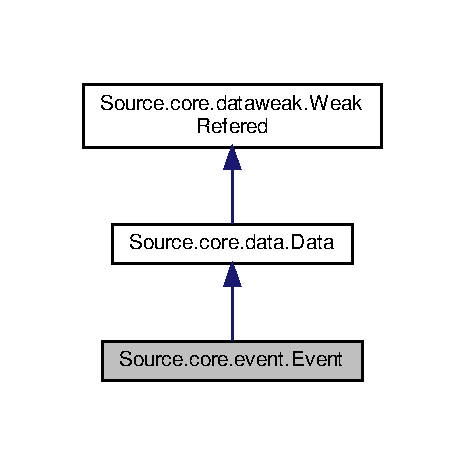
\includegraphics[width=223pt]{classSource_1_1core_1_1event_1_1Event__inherit__graph}
\end{center}
\end{figure}


Collaboration diagram for Source.\+core.\+event.\+Event\+:\nopagebreak
\begin{figure}[H]
\begin{center}
\leavevmode
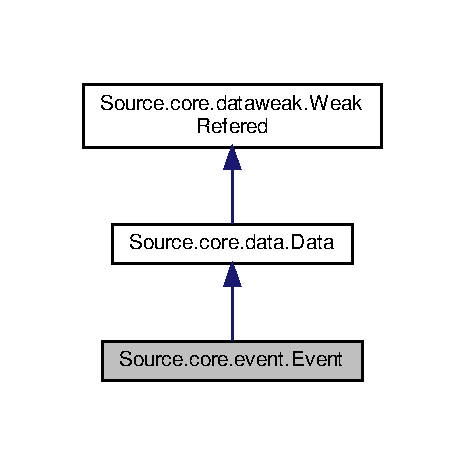
\includegraphics[width=223pt]{classSource_1_1core_1_1event_1_1Event__coll__graph}
\end{center}
\end{figure}
\subsection*{Public Member Functions}
\begin{DoxyCompactItemize}
\item 
def \mbox{\hyperlink{classSource_1_1core_1_1event_1_1Event_aa661baba9387dbb7b60fc6d90028dc2a}{\+\_\+\+\_\+init\+\_\+\+\_\+}} (self, \+\_\+id, collection, start, end, type, description, resources, users, agenda=None, creation\+\_\+date=None)
\begin{DoxyCompactList}\small\item\em Création d\textquotesingle{}un évènement. \end{DoxyCompactList}\item 
def \mbox{\hyperlink{classSource_1_1core_1_1event_1_1Event_ac97a1c0a1f4e7b5a96d4584c6c623f75}{update}} (self)
\begin{DoxyCompactList}\small\item\em Actualisation de la date de dernière modification. \end{DoxyCompactList}\item 
\mbox{\Hypertarget{classSource_1_1core_1_1event_1_1Event_a60d7defd3e3d2af8764016d376d94433}\label{classSource_1_1core_1_1event_1_1Event_a60d7defd3e3d2af8764016d376d94433}} 
def \mbox{\hyperlink{classSource_1_1core_1_1event_1_1Event_a60d7defd3e3d2af8764016d376d94433}{duration}} (self)
\begin{DoxyCompactList}\small\item\em return la durée de l\textquotesingle{}évènement \end{DoxyCompactList}\item 
\mbox{\Hypertarget{classSource_1_1core_1_1event_1_1Event_a3fd82af192d7dacd5daffcb4945fa40d}\label{classSource_1_1core_1_1event_1_1Event_a3fd82af192d7dacd5daffcb4945fa40d}} 
def \mbox{\hyperlink{classSource_1_1core_1_1event_1_1Event_a3fd82af192d7dacd5daffcb4945fa40d}{add\+\_\+user}} (self, user)
\begin{DoxyCompactList}\small\item\em Ajout d\textquotesingle{}un utilisateur sur un event. \end{DoxyCompactList}\item 
\mbox{\Hypertarget{classSource_1_1core_1_1event_1_1Event_af65b6800b73ce8b9c101d26aa0692360}\label{classSource_1_1core_1_1event_1_1Event_af65b6800b73ce8b9c101d26aa0692360}} 
def \mbox{\hyperlink{classSource_1_1core_1_1event_1_1Event_af65b6800b73ce8b9c101d26aa0692360}{remove\+\_\+user}} (self, user)
\begin{DoxyCompactList}\small\item\em suppression de la participation d\textquotesingle{}un utilisateur à un évènement \end{DoxyCompactList}\item 
\mbox{\Hypertarget{classSource_1_1core_1_1event_1_1Event_ae197fc2b7904a8b564da48208da1e78b}\label{classSource_1_1core_1_1event_1_1Event_ae197fc2b7904a8b564da48208da1e78b}} 
def \mbox{\hyperlink{classSource_1_1core_1_1event_1_1Event_ae197fc2b7904a8b564da48208da1e78b}{add\+\_\+resource}} (self, resource)
\begin{DoxyCompactList}\small\item\em Ajout d\textquotesingle{}une ressource pour un event. \end{DoxyCompactList}\item 
\mbox{\Hypertarget{classSource_1_1core_1_1event_1_1Event_a7162c0262b2c90d79e0b84e6f92b4115}\label{classSource_1_1core_1_1event_1_1Event_a7162c0262b2c90d79e0b84e6f92b4115}} 
def \mbox{\hyperlink{classSource_1_1core_1_1event_1_1Event_a7162c0262b2c90d79e0b84e6f92b4115}{remove\+\_\+resource}} (self, resource)
\begin{DoxyCompactList}\small\item\em Suppression d\textquotesingle{}une ressource pour un event. \end{DoxyCompactList}\item 
\mbox{\Hypertarget{classSource_1_1core_1_1event_1_1Event_abb47ab9b43b636aa0bb781954d9e23ec}\label{classSource_1_1core_1_1event_1_1Event_abb47ab9b43b636aa0bb781954d9e23ec}} 
def {\bfseries intersect} (self, event)
\item 
\mbox{\Hypertarget{classSource_1_1core_1_1event_1_1Event_af71ff5b923f293bae949cbfd45f31cb4}\label{classSource_1_1core_1_1event_1_1Event_af71ff5b923f293bae949cbfd45f31cb4}} 
def \mbox{\hyperlink{classSource_1_1core_1_1event_1_1Event_af71ff5b923f293bae949cbfd45f31cb4}{\+\_\+\+\_\+repr\+\_\+\+\_\+}} (self)
\begin{DoxyCompactList}\small\item\em affiche l\textquotesingle{}event \end{DoxyCompactList}\end{DoxyCompactItemize}
\subsection*{Public Attributes}
\begin{DoxyCompactItemize}
\item 
\mbox{\Hypertarget{classSource_1_1core_1_1event_1_1Event_a3e2d19a56e162169c6ea568ea8d8efd4}\label{classSource_1_1core_1_1event_1_1Event_a3e2d19a56e162169c6ea568ea8d8efd4}} 
{\bfseries resources}
\item 
\mbox{\Hypertarget{classSource_1_1core_1_1event_1_1Event_a8a1b2f9cf2b7cf5f8785f0784aea8b66}\label{classSource_1_1core_1_1event_1_1Event_a8a1b2f9cf2b7cf5f8785f0784aea8b66}} 
{\bfseries users}
\end{DoxyCompactItemize}
\subsection*{Static Public Attributes}
\begin{DoxyCompactItemize}
\item 
\mbox{\Hypertarget{classSource_1_1core_1_1event_1_1Event_abc2dafb4e695c82d8200d9fa2d57718d}\label{classSource_1_1core_1_1event_1_1Event_abc2dafb4e695c82d8200d9fa2d57718d}} 
{\bfseries start} = \mbox{\hyperlink{classSource_1_1core_1_1dataproperty_1_1DataProperty}{Data\+Property}}(\char`\"{}start\char`\"{})
\item 
\mbox{\Hypertarget{classSource_1_1core_1_1event_1_1Event_a4c0a6edca4531d80a03b1dd7662edd7c}\label{classSource_1_1core_1_1event_1_1Event_a4c0a6edca4531d80a03b1dd7662edd7c}} 
{\bfseries end} = \mbox{\hyperlink{classSource_1_1core_1_1dataproperty_1_1DataProperty}{Data\+Property}}(\char`\"{}end\char`\"{})
\item 
\mbox{\Hypertarget{classSource_1_1core_1_1event_1_1Event_aae2b1359f1cd50db08df27a2e6f036e2}\label{classSource_1_1core_1_1event_1_1Event_aae2b1359f1cd50db08df27a2e6f036e2}} 
{\bfseries type} = \mbox{\hyperlink{classSource_1_1core_1_1dataproperty_1_1DataProperty}{Data\+Property}}(\char`\"{}type\char`\"{})
\item 
\mbox{\Hypertarget{classSource_1_1core_1_1event_1_1Event_acaec09233730afab11bbf952079d62bc}\label{classSource_1_1core_1_1event_1_1Event_acaec09233730afab11bbf952079d62bc}} 
{\bfseries description} = \mbox{\hyperlink{classSource_1_1core_1_1dataproperty_1_1DataProperty}{Data\+Property}}(\char`\"{}description\char`\"{})
\item 
\mbox{\Hypertarget{classSource_1_1core_1_1event_1_1Event_a7e87516be7f4e4f76ce36c899f7c1093}\label{classSource_1_1core_1_1event_1_1Event_a7e87516be7f4e4f76ce36c899f7c1093}} 
{\bfseries agenda} = \mbox{\hyperlink{classSource_1_1core_1_1dataproperty_1_1DataOwnerProperty}{Data\+Owner\+Property}}(\char`\"{}agenda\char`\"{})
\item 
\mbox{\Hypertarget{classSource_1_1core_1_1event_1_1Event_af242c5f37256e19fc14530215c939dec}\label{classSource_1_1core_1_1event_1_1Event_af242c5f37256e19fc14530215c939dec}} 
{\bfseries creation\+\_\+date} = \mbox{\hyperlink{classSource_1_1core_1_1dataproperty_1_1DataProperty}{Data\+Property}}(\char`\"{}creation\+\_\+date\char`\"{})
\end{DoxyCompactItemize}


\subsection{Constructor \& Destructor Documentation}
\mbox{\Hypertarget{classSource_1_1core_1_1event_1_1Event_aa661baba9387dbb7b60fc6d90028dc2a}\label{classSource_1_1core_1_1event_1_1Event_aa661baba9387dbb7b60fc6d90028dc2a}} 
\index{Source\+::core\+::event\+::\+Event@{Source\+::core\+::event\+::\+Event}!\+\_\+\+\_\+init\+\_\+\+\_\+@{\+\_\+\+\_\+init\+\_\+\+\_\+}}
\index{\+\_\+\+\_\+init\+\_\+\+\_\+@{\+\_\+\+\_\+init\+\_\+\+\_\+}!Source\+::core\+::event\+::\+Event@{Source\+::core\+::event\+::\+Event}}
\subsubsection{\texorpdfstring{\+\_\+\+\_\+init\+\_\+\+\_\+()}{\_\_init\_\_()}}
{\footnotesize\ttfamily def Source.\+core.\+event.\+Event.\+\_\+\+\_\+init\+\_\+\+\_\+ (\begin{DoxyParamCaption}\item[{}]{self,  }\item[{}]{\+\_\+id,  }\item[{}]{collection,  }\item[{}]{start,  }\item[{}]{end,  }\item[{}]{type,  }\item[{}]{description,  }\item[{}]{resources,  }\item[{}]{users,  }\item[{}]{agenda = {\ttfamily None},  }\item[{}]{creation\+\_\+date = {\ttfamily None} }\end{DoxyParamCaption})}



Création d\textquotesingle{}un évènement. 


\begin{DoxyParams}{Parameters}
{\em collection} & \+: la collection à passer (dans le fichier common). ... \\
\hline
\end{DoxyParams}


\subsection{Member Function Documentation}
\mbox{\Hypertarget{classSource_1_1core_1_1event_1_1Event_ac97a1c0a1f4e7b5a96d4584c6c623f75}\label{classSource_1_1core_1_1event_1_1Event_ac97a1c0a1f4e7b5a96d4584c6c623f75}} 
\index{Source\+::core\+::event\+::\+Event@{Source\+::core\+::event\+::\+Event}!update@{update}}
\index{update@{update}!Source\+::core\+::event\+::\+Event@{Source\+::core\+::event\+::\+Event}}
\subsubsection{\texorpdfstring{update()}{update()}}
{\footnotesize\ttfamily def Source.\+core.\+event.\+Event.\+update (\begin{DoxyParamCaption}\item[{}]{self }\end{DoxyParamCaption})}



Actualisation de la date de dernière modification. 



The documentation for this class was generated from the following file\+:\begin{DoxyCompactItemize}
\item 
/home/tristan/\+Documents/\+U\+S\+M\+B/\+I\+N\+F\+O\+\_\+406/\+Source/core/event.\+py\end{DoxyCompactItemize}

\hypertarget{classSource_1_1core_1_1group_1_1Group}{}\section{Source.\+core.\+group.\+Group Class Reference}
\label{classSource_1_1core_1_1group_1_1Group}\index{Source.\+core.\+group.\+Group@{Source.\+core.\+group.\+Group}}


Inheritance diagram for Source.\+core.\+group.\+Group\+:\nopagebreak
\begin{figure}[H]
\begin{center}
\leavevmode
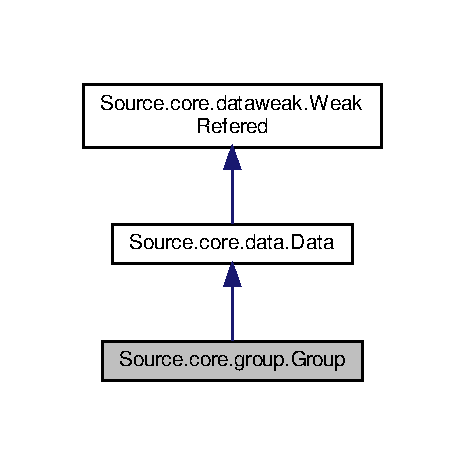
\includegraphics[width=223pt]{classSource_1_1core_1_1group_1_1Group__inherit__graph}
\end{center}
\end{figure}


Collaboration diagram for Source.\+core.\+group.\+Group\+:\nopagebreak
\begin{figure}[H]
\begin{center}
\leavevmode
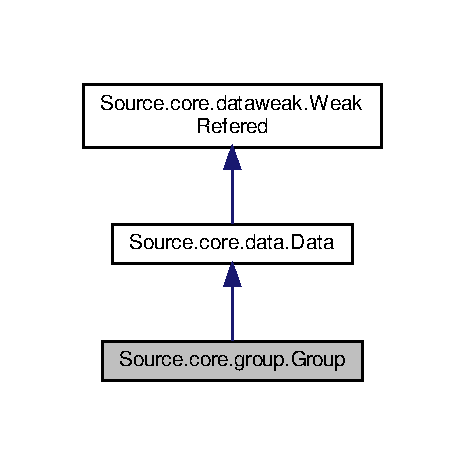
\includegraphics[width=223pt]{classSource_1_1core_1_1group_1_1Group__coll__graph}
\end{center}
\end{figure}
\subsection*{Public Member Functions}
\begin{DoxyCompactItemize}
\item 
\mbox{\Hypertarget{classSource_1_1core_1_1group_1_1Group_a9243664238a587738f4477dd43e1f688}\label{classSource_1_1core_1_1group_1_1Group_a9243664238a587738f4477dd43e1f688}} 
def {\bfseries \+\_\+\+\_\+init\+\_\+\+\_\+} (self, \+\_\+id, collection, name, admins, subscribers, agendas, resources)
\item 
\mbox{\Hypertarget{classSource_1_1core_1_1group_1_1Group_a8993ec36f5da4b5ed248c193717eb5bd}\label{classSource_1_1core_1_1group_1_1Group_a8993ec36f5da4b5ed248c193717eb5bd}} 
def {\bfseries \+\_\+\+\_\+repr\+\_\+\+\_\+} (self)
\item 
def \mbox{\hyperlink{classSource_1_1core_1_1group_1_1Group_ad778ec8b8e391fdada7ed5c1843ab1e1}{add\+\_\+agenda}} (self, agenda)
\begin{DoxyCompactList}\small\item\em Ajout d\textquotesingle{}un agenda. \end{DoxyCompactList}\item 
def \mbox{\hyperlink{classSource_1_1core_1_1group_1_1Group_ad9acb8c0acca1abf60bba16d21bb60a3}{remove\+\_\+agenda}} (self, agenda)
\begin{DoxyCompactList}\small\item\em Suppression d\textquotesingle{}un agenda de la liste. \end{DoxyCompactList}\item 
def \mbox{\hyperlink{classSource_1_1core_1_1group_1_1Group_a92e2cdd12d4220411d1e6990efe46ab4}{subscribe}} (self, user)
\begin{DoxyCompactList}\small\item\em Inscription d\textquotesingle{}un utilisateur. \end{DoxyCompactList}\item 
def \mbox{\hyperlink{classSource_1_1core_1_1group_1_1Group_a0ceabbe4c3cadd23a63628c8aa08023f}{unsubscribe}} (self, user)
\begin{DoxyCompactList}\small\item\em Desinscription d\textquotesingle{}un utilisateur. \end{DoxyCompactList}\item 
def \mbox{\hyperlink{classSource_1_1core_1_1group_1_1Group_aef733eb961bc40234c9c1612844f3708}{is\+\_\+admin}} (self, user)
\begin{DoxyCompactList}\small\item\em Test si un utilisateur est administrateur. \end{DoxyCompactList}\item 
def \mbox{\hyperlink{classSource_1_1core_1_1group_1_1Group_abf48501aa3d976ca92e2ea3194633b12}{add\+\_\+admin}} (self, user)
\begin{DoxyCompactList}\small\item\em Ajout d\textquotesingle{}un administrateur. \end{DoxyCompactList}\item 
def \mbox{\hyperlink{classSource_1_1core_1_1group_1_1Group_a08ca8a3d7a46d06841e454094b0d3504}{remove\+\_\+admin}} (self, user)
\begin{DoxyCompactList}\small\item\em Suppression d\textquotesingle{}un administrateur. \end{DoxyCompactList}\end{DoxyCompactItemize}
\subsection*{Public Attributes}
\begin{DoxyCompactItemize}
\item 
\mbox{\Hypertarget{classSource_1_1core_1_1group_1_1Group_a68ae845c5772685e8cf75122f3472b9c}\label{classSource_1_1core_1_1group_1_1Group_a68ae845c5772685e8cf75122f3472b9c}} 
{\bfseries admins}
\item 
\mbox{\Hypertarget{classSource_1_1core_1_1group_1_1Group_abcd27cfb7adc97cef9bee0f89b8e1165}\label{classSource_1_1core_1_1group_1_1Group_abcd27cfb7adc97cef9bee0f89b8e1165}} 
{\bfseries subscribers}
\item 
\mbox{\Hypertarget{classSource_1_1core_1_1group_1_1Group_ae553c76b852a126b4f35ee56427ab39d}\label{classSource_1_1core_1_1group_1_1Group_ae553c76b852a126b4f35ee56427ab39d}} 
{\bfseries agendas}
\item 
\mbox{\Hypertarget{classSource_1_1core_1_1group_1_1Group_a900634df8eb7a5e4a0e03e3f5eca8d7a}\label{classSource_1_1core_1_1group_1_1Group_a900634df8eb7a5e4a0e03e3f5eca8d7a}} 
{\bfseries resources}
\end{DoxyCompactItemize}
\subsection*{Static Public Attributes}
\begin{DoxyCompactItemize}
\item 
\mbox{\Hypertarget{classSource_1_1core_1_1group_1_1Group_a7b142a5a7f8c054977bff8b2fd36ac18}\label{classSource_1_1core_1_1group_1_1Group_a7b142a5a7f8c054977bff8b2fd36ac18}} 
{\bfseries name} = \mbox{\hyperlink{classSource_1_1core_1_1dataproperty_1_1DataProperty}{Data\+Property}}(\char`\"{}name\char`\"{})
\end{DoxyCompactItemize}


\subsection{Member Function Documentation}
\mbox{\Hypertarget{classSource_1_1core_1_1group_1_1Group_abf48501aa3d976ca92e2ea3194633b12}\label{classSource_1_1core_1_1group_1_1Group_abf48501aa3d976ca92e2ea3194633b12}} 
\index{Source\+::core\+::group\+::\+Group@{Source\+::core\+::group\+::\+Group}!add\+\_\+admin@{add\+\_\+admin}}
\index{add\+\_\+admin@{add\+\_\+admin}!Source\+::core\+::group\+::\+Group@{Source\+::core\+::group\+::\+Group}}
\subsubsection{\texorpdfstring{add\+\_\+admin()}{add\_admin()}}
{\footnotesize\ttfamily def Source.\+core.\+group.\+Group.\+add\+\_\+admin (\begin{DoxyParamCaption}\item[{}]{self,  }\item[{}]{user }\end{DoxyParamCaption})}



Ajout d\textquotesingle{}un administrateur. 

\mbox{\Hypertarget{classSource_1_1core_1_1group_1_1Group_ad778ec8b8e391fdada7ed5c1843ab1e1}\label{classSource_1_1core_1_1group_1_1Group_ad778ec8b8e391fdada7ed5c1843ab1e1}} 
\index{Source\+::core\+::group\+::\+Group@{Source\+::core\+::group\+::\+Group}!add\+\_\+agenda@{add\+\_\+agenda}}
\index{add\+\_\+agenda@{add\+\_\+agenda}!Source\+::core\+::group\+::\+Group@{Source\+::core\+::group\+::\+Group}}
\subsubsection{\texorpdfstring{add\+\_\+agenda()}{add\_agenda()}}
{\footnotesize\ttfamily def Source.\+core.\+group.\+Group.\+add\+\_\+agenda (\begin{DoxyParamCaption}\item[{}]{self,  }\item[{}]{agenda }\end{DoxyParamCaption})}



Ajout d\textquotesingle{}un agenda. 

\mbox{\Hypertarget{classSource_1_1core_1_1group_1_1Group_aef733eb961bc40234c9c1612844f3708}\label{classSource_1_1core_1_1group_1_1Group_aef733eb961bc40234c9c1612844f3708}} 
\index{Source\+::core\+::group\+::\+Group@{Source\+::core\+::group\+::\+Group}!is\+\_\+admin@{is\+\_\+admin}}
\index{is\+\_\+admin@{is\+\_\+admin}!Source\+::core\+::group\+::\+Group@{Source\+::core\+::group\+::\+Group}}
\subsubsection{\texorpdfstring{is\+\_\+admin()}{is\_admin()}}
{\footnotesize\ttfamily def Source.\+core.\+group.\+Group.\+is\+\_\+admin (\begin{DoxyParamCaption}\item[{}]{self,  }\item[{}]{user }\end{DoxyParamCaption})}



Test si un utilisateur est administrateur. 

\mbox{\Hypertarget{classSource_1_1core_1_1group_1_1Group_a08ca8a3d7a46d06841e454094b0d3504}\label{classSource_1_1core_1_1group_1_1Group_a08ca8a3d7a46d06841e454094b0d3504}} 
\index{Source\+::core\+::group\+::\+Group@{Source\+::core\+::group\+::\+Group}!remove\+\_\+admin@{remove\+\_\+admin}}
\index{remove\+\_\+admin@{remove\+\_\+admin}!Source\+::core\+::group\+::\+Group@{Source\+::core\+::group\+::\+Group}}
\subsubsection{\texorpdfstring{remove\+\_\+admin()}{remove\_admin()}}
{\footnotesize\ttfamily def Source.\+core.\+group.\+Group.\+remove\+\_\+admin (\begin{DoxyParamCaption}\item[{}]{self,  }\item[{}]{user }\end{DoxyParamCaption})}



Suppression d\textquotesingle{}un administrateur. 

\mbox{\Hypertarget{classSource_1_1core_1_1group_1_1Group_ad9acb8c0acca1abf60bba16d21bb60a3}\label{classSource_1_1core_1_1group_1_1Group_ad9acb8c0acca1abf60bba16d21bb60a3}} 
\index{Source\+::core\+::group\+::\+Group@{Source\+::core\+::group\+::\+Group}!remove\+\_\+agenda@{remove\+\_\+agenda}}
\index{remove\+\_\+agenda@{remove\+\_\+agenda}!Source\+::core\+::group\+::\+Group@{Source\+::core\+::group\+::\+Group}}
\subsubsection{\texorpdfstring{remove\+\_\+agenda()}{remove\_agenda()}}
{\footnotesize\ttfamily def Source.\+core.\+group.\+Group.\+remove\+\_\+agenda (\begin{DoxyParamCaption}\item[{}]{self,  }\item[{}]{agenda }\end{DoxyParamCaption})}



Suppression d\textquotesingle{}un agenda de la liste. 

\mbox{\Hypertarget{classSource_1_1core_1_1group_1_1Group_a92e2cdd12d4220411d1e6990efe46ab4}\label{classSource_1_1core_1_1group_1_1Group_a92e2cdd12d4220411d1e6990efe46ab4}} 
\index{Source\+::core\+::group\+::\+Group@{Source\+::core\+::group\+::\+Group}!subscribe@{subscribe}}
\index{subscribe@{subscribe}!Source\+::core\+::group\+::\+Group@{Source\+::core\+::group\+::\+Group}}
\subsubsection{\texorpdfstring{subscribe()}{subscribe()}}
{\footnotesize\ttfamily def Source.\+core.\+group.\+Group.\+subscribe (\begin{DoxyParamCaption}\item[{}]{self,  }\item[{}]{user }\end{DoxyParamCaption})}



Inscription d\textquotesingle{}un utilisateur. 

\mbox{\Hypertarget{classSource_1_1core_1_1group_1_1Group_a0ceabbe4c3cadd23a63628c8aa08023f}\label{classSource_1_1core_1_1group_1_1Group_a0ceabbe4c3cadd23a63628c8aa08023f}} 
\index{Source\+::core\+::group\+::\+Group@{Source\+::core\+::group\+::\+Group}!unsubscribe@{unsubscribe}}
\index{unsubscribe@{unsubscribe}!Source\+::core\+::group\+::\+Group@{Source\+::core\+::group\+::\+Group}}
\subsubsection{\texorpdfstring{unsubscribe()}{unsubscribe()}}
{\footnotesize\ttfamily def Source.\+core.\+group.\+Group.\+unsubscribe (\begin{DoxyParamCaption}\item[{}]{self,  }\item[{}]{user }\end{DoxyParamCaption})}



Desinscription d\textquotesingle{}un utilisateur. 



The documentation for this class was generated from the following file\+:\begin{DoxyCompactItemize}
\item 
/home/tristan/\+Documents/\+U\+S\+M\+B/\+I\+N\+F\+O\+\_\+406/\+Source/core/group.\+py\end{DoxyCompactItemize}

\hypertarget{classSource_1_1core_1_1notification_1_1Notification}{}\section{Source.\+core.\+notification.\+Notification Class Reference}
\label{classSource_1_1core_1_1notification_1_1Notification}\index{Source.\+core.\+notification.\+Notification@{Source.\+core.\+notification.\+Notification}}


Inheritance diagram for Source.\+core.\+notification.\+Notification\+:\nopagebreak
\begin{figure}[H]
\begin{center}
\leavevmode
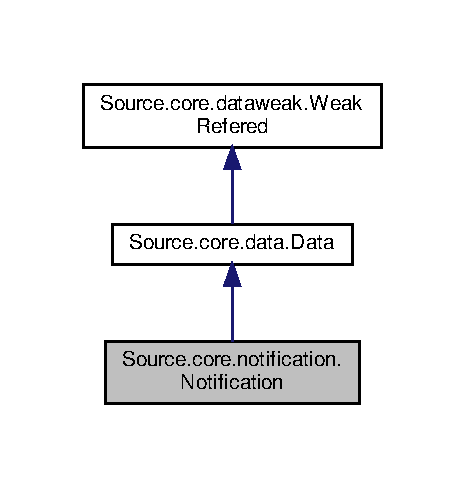
\includegraphics[width=223pt]{classSource_1_1core_1_1notification_1_1Notification__inherit__graph}
\end{center}
\end{figure}


Collaboration diagram for Source.\+core.\+notification.\+Notification\+:\nopagebreak
\begin{figure}[H]
\begin{center}
\leavevmode
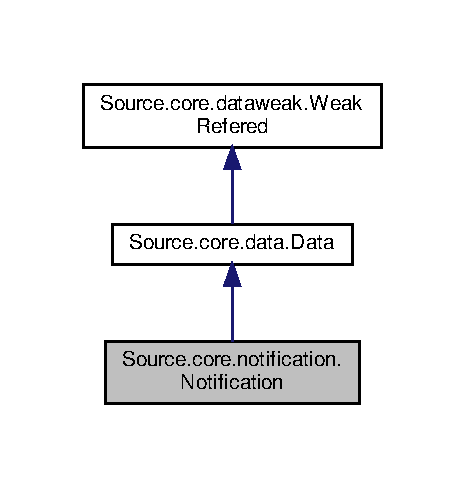
\includegraphics[width=223pt]{classSource_1_1core_1_1notification_1_1Notification__coll__graph}
\end{center}
\end{figure}
\subsection*{Public Member Functions}
\begin{DoxyCompactItemize}
\item 
\mbox{\Hypertarget{classSource_1_1core_1_1notification_1_1Notification_a957251915d6f26f621420f3a9eaff192}\label{classSource_1_1core_1_1notification_1_1Notification_a957251915d6f26f621420f3a9eaff192}} 
def {\bfseries \+\_\+\+\_\+init\+\_\+\+\_\+} (self, \+\_\+id, collection, event, agenda, status)
\item 
\mbox{\Hypertarget{classSource_1_1core_1_1notification_1_1Notification_a7ab07601c90618e04325cfdacf0cd308}\label{classSource_1_1core_1_1notification_1_1Notification_a7ab07601c90618e04325cfdacf0cd308}} 
def {\bfseries \+\_\+\+\_\+repr\+\_\+\+\_\+} (self)
\end{DoxyCompactItemize}
\subsection*{Static Public Attributes}
\begin{DoxyCompactItemize}
\item 
\mbox{\Hypertarget{classSource_1_1core_1_1notification_1_1Notification_a7ea11d6511202bc217ac991722fd3430}\label{classSource_1_1core_1_1notification_1_1Notification_a7ea11d6511202bc217ac991722fd3430}} 
{\bfseries event} = \mbox{\hyperlink{classSource_1_1core_1_1dataproperty_1_1DataOwnerProperty}{Data\+Owner\+Property}}(\char`\"{}event\char`\"{})
\item 
\mbox{\Hypertarget{classSource_1_1core_1_1notification_1_1Notification_aff5ae8ab5c5bf7a8d539a2d39b0a831a}\label{classSource_1_1core_1_1notification_1_1Notification_aff5ae8ab5c5bf7a8d539a2d39b0a831a}} 
{\bfseries agenda} = \mbox{\hyperlink{classSource_1_1core_1_1dataproperty_1_1DataOwnerProperty}{Data\+Owner\+Property}}(\char`\"{}agenda\char`\"{})
\item 
\mbox{\Hypertarget{classSource_1_1core_1_1notification_1_1Notification_a3cd653af18a24b8ebdd2a54fb83aec05}\label{classSource_1_1core_1_1notification_1_1Notification_a3cd653af18a24b8ebdd2a54fb83aec05}} 
{\bfseries status} = \mbox{\hyperlink{classSource_1_1core_1_1dataproperty_1_1DataOwnerProperty}{Data\+Owner\+Property}}(\char`\"{}status\char`\"{})
\end{DoxyCompactItemize}
\subsection*{Additional Inherited Members}


The documentation for this class was generated from the following file\+:\begin{DoxyCompactItemize}
\item 
/home/tristan/\+Documents/\+U\+S\+M\+B/\+I\+N\+F\+O\+\_\+406/\+Source/core/notification.\+py\end{DoxyCompactItemize}

\hypertarget{classSource_1_1core_1_1presence_1_1Presence}{}\section{Source.\+core.\+presence.\+Presence Class Reference}
\label{classSource_1_1core_1_1presence_1_1Presence}\index{Source.\+core.\+presence.\+Presence@{Source.\+core.\+presence.\+Presence}}
\subsection*{Public Member Functions}
\begin{DoxyCompactItemize}
\item 
\mbox{\Hypertarget{classSource_1_1core_1_1presence_1_1Presence_a5506dc5242f9fb6e27af5a07b2aecf80}\label{classSource_1_1core_1_1presence_1_1Presence_a5506dc5242f9fb6e27af5a07b2aecf80}} 
def {\bfseries \+\_\+\+\_\+init\+\_\+\+\_\+} (self, slot, users)
\item 
\mbox{\Hypertarget{classSource_1_1core_1_1presence_1_1Presence_ae7309791615cbaf84bcb9d35aabf4908}\label{classSource_1_1core_1_1presence_1_1Presence_ae7309791615cbaf84bcb9d35aabf4908}} 
def {\bfseries \+\_\+\+\_\+repr\+\_\+\+\_\+} (self)
\end{DoxyCompactItemize}
\subsection*{Public Attributes}
\begin{DoxyCompactItemize}
\item 
\mbox{\Hypertarget{classSource_1_1core_1_1presence_1_1Presence_ab0efc367b62008645e1db05a507d004b}\label{classSource_1_1core_1_1presence_1_1Presence_ab0efc367b62008645e1db05a507d004b}} 
{\bfseries slot}
\item 
\mbox{\Hypertarget{classSource_1_1core_1_1presence_1_1Presence_a0871b8495e93e6cb785fbbc4f396114d}\label{classSource_1_1core_1_1presence_1_1Presence_a0871b8495e93e6cb785fbbc4f396114d}} 
{\bfseries users}
\end{DoxyCompactItemize}


The documentation for this class was generated from the following file\+:\begin{DoxyCompactItemize}
\item 
/home/tristan/\+Documents/\+U\+S\+M\+B/\+I\+N\+F\+O\+\_\+406/\+Source/core/presence.\+py\end{DoxyCompactItemize}

\hypertarget{classproperty}{}\section{property Class Reference}
\label{classproperty}\index{property@{property}}


Inheritance diagram for property\+:\nopagebreak
\begin{figure}[H]
\begin{center}
\leavevmode
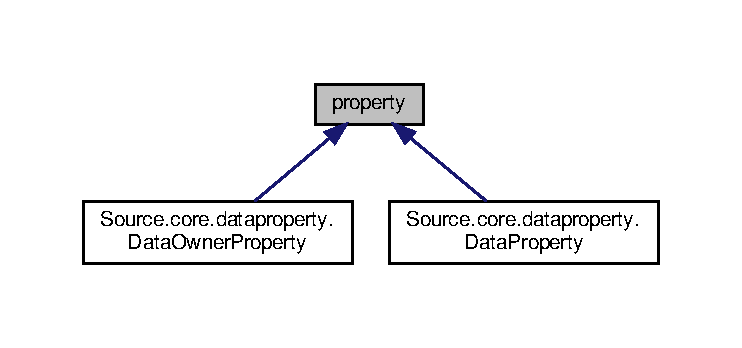
\includegraphics[width=350pt]{classproperty__inherit__graph}
\end{center}
\end{figure}


The documentation for this class was generated from the following file\+:\begin{DoxyCompactItemize}
\item 
/home/tristan/\+Documents/\+U\+S\+M\+B/\+I\+N\+F\+O\+\_\+406/\+Source/core/dataproperty.\+py\end{DoxyCompactItemize}

\hypertarget{classSource_1_1core_1_1resource_1_1Resource}{}\section{Source.\+core.\+resource.\+Resource Class Reference}
\label{classSource_1_1core_1_1resource_1_1Resource}\index{Source.\+core.\+resource.\+Resource@{Source.\+core.\+resource.\+Resource}}


Inheritance diagram for Source.\+core.\+resource.\+Resource\+:\nopagebreak
\begin{figure}[H]
\begin{center}
\leavevmode
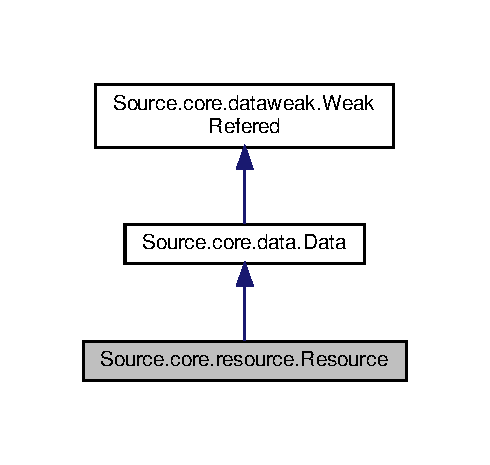
\includegraphics[width=235pt]{classSource_1_1core_1_1resource_1_1Resource__inherit__graph}
\end{center}
\end{figure}


Collaboration diagram for Source.\+core.\+resource.\+Resource\+:\nopagebreak
\begin{figure}[H]
\begin{center}
\leavevmode
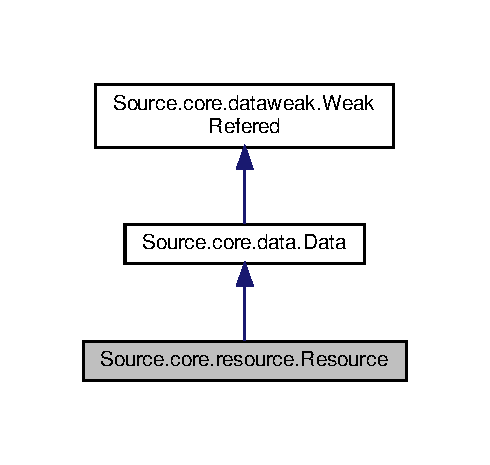
\includegraphics[width=235pt]{classSource_1_1core_1_1resource_1_1Resource__coll__graph}
\end{center}
\end{figure}
\subsection*{Public Member Functions}
\begin{DoxyCompactItemize}
\item 
\mbox{\Hypertarget{classSource_1_1core_1_1resource_1_1Resource_a1d4a67c41ffbf552a7930efa53b649d1}\label{classSource_1_1core_1_1resource_1_1Resource_a1d4a67c41ffbf552a7930efa53b649d1}} 
def {\bfseries \+\_\+\+\_\+init\+\_\+\+\_\+} (self, \+\_\+id, collection, name, location, capacity, group)
\end{DoxyCompactItemize}
\subsection*{Static Public Attributes}
\begin{DoxyCompactItemize}
\item 
\mbox{\Hypertarget{classSource_1_1core_1_1resource_1_1Resource_aa7442c19118b55022614af28009c9aef}\label{classSource_1_1core_1_1resource_1_1Resource_aa7442c19118b55022614af28009c9aef}} 
{\bfseries name} = \mbox{\hyperlink{classSource_1_1core_1_1dataproperty_1_1DataProperty}{Data\+Property}}(\char`\"{}name\char`\"{})
\item 
\mbox{\Hypertarget{classSource_1_1core_1_1resource_1_1Resource_adda385d0e316dfb2bdec55889f030166}\label{classSource_1_1core_1_1resource_1_1Resource_adda385d0e316dfb2bdec55889f030166}} 
{\bfseries location} = \mbox{\hyperlink{classSource_1_1core_1_1dataproperty_1_1DataProperty}{Data\+Property}}(\char`\"{}location\char`\"{})
\item 
\mbox{\Hypertarget{classSource_1_1core_1_1resource_1_1Resource_a1e3aaabaa9676995cf80741ca85952a2}\label{classSource_1_1core_1_1resource_1_1Resource_a1e3aaabaa9676995cf80741ca85952a2}} 
{\bfseries capacity} = \mbox{\hyperlink{classSource_1_1core_1_1dataproperty_1_1DataProperty}{Data\+Property}}(\char`\"{}capacity\char`\"{})
\item 
\mbox{\Hypertarget{classSource_1_1core_1_1resource_1_1Resource_afafd9b0001684bcab9a126ee4f632e6f}\label{classSource_1_1core_1_1resource_1_1Resource_afafd9b0001684bcab9a126ee4f632e6f}} 
{\bfseries group} = \mbox{\hyperlink{classSource_1_1core_1_1dataproperty_1_1DataOwnerProperty}{Data\+Owner\+Property}}(\char`\"{}group\char`\"{})
\end{DoxyCompactItemize}
\subsection*{Additional Inherited Members}


The documentation for this class was generated from the following file\+:\begin{DoxyCompactItemize}
\item 
/home/tristan/\+Documents/\+U\+S\+M\+B/\+I\+N\+F\+O\+\_\+406/\+Source/core/resource.\+py\end{DoxyCompactItemize}

\hypertarget{classSource_1_1core_1_1user_1_1User}{}\section{Source.\+core.\+user.\+User Class Reference}
\label{classSource_1_1core_1_1user_1_1User}\index{Source.\+core.\+user.\+User@{Source.\+core.\+user.\+User}}


Inheritance diagram for Source.\+core.\+user.\+User\+:\nopagebreak
\begin{figure}[H]
\begin{center}
\leavevmode
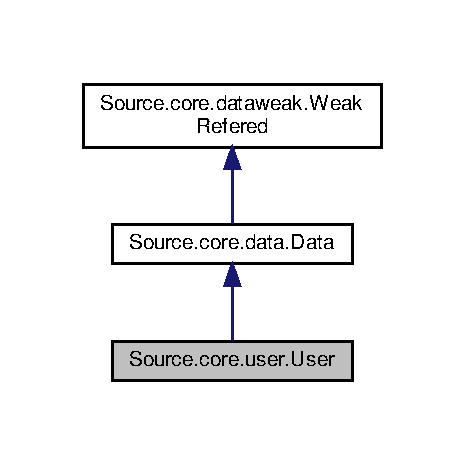
\includegraphics[width=223pt]{classSource_1_1core_1_1user_1_1User__inherit__graph}
\end{center}
\end{figure}


Collaboration diagram for Source.\+core.\+user.\+User\+:\nopagebreak
\begin{figure}[H]
\begin{center}
\leavevmode
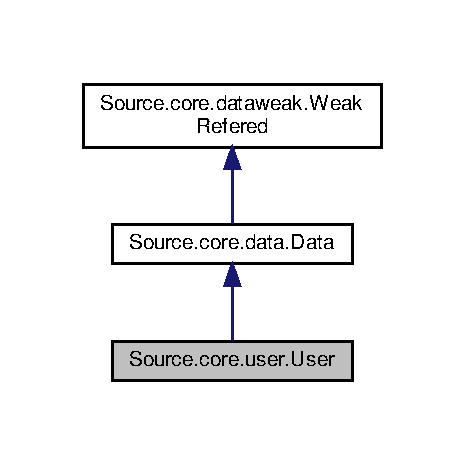
\includegraphics[width=223pt]{classSource_1_1core_1_1user_1_1User__coll__graph}
\end{center}
\end{figure}
\subsection*{Public Member Functions}
\begin{DoxyCompactItemize}
\item 
\mbox{\Hypertarget{classSource_1_1core_1_1user_1_1User_a8d29da6a2ae1876c27166f3faf2dc1c6}\label{classSource_1_1core_1_1user_1_1User_a8d29da6a2ae1876c27166f3faf2dc1c6}} 
def \mbox{\hyperlink{classSource_1_1core_1_1user_1_1User_a8d29da6a2ae1876c27166f3faf2dc1c6}{\+\_\+\+\_\+init\+\_\+\+\_\+}} (self, \+\_\+id, collection, first\+\_\+name, last\+\_\+name, email, tel, \mbox{\hyperlink{classSource_1_1core_1_1user_1_1User_aca59c238ba182f8409f6c9c37b3b9e9b}{agenda}}, groups, account=None)
\begin{DoxyCompactList}\small\item\em création d\textquotesingle{}un utilisate \end{DoxyCompactList}\item 
\mbox{\Hypertarget{classSource_1_1core_1_1user_1_1User_a73a5a2e042cce83c61bf3b10ebb0db6c}\label{classSource_1_1core_1_1user_1_1User_a73a5a2e042cce83c61bf3b10ebb0db6c}} 
def {\bfseries \+\_\+\+\_\+repr\+\_\+\+\_\+} (self)
\item 
\mbox{\Hypertarget{classSource_1_1core_1_1user_1_1User_aca59c238ba182f8409f6c9c37b3b9e9b}\label{classSource_1_1core_1_1user_1_1User_aca59c238ba182f8409f6c9c37b3b9e9b}} 
def \mbox{\hyperlink{classSource_1_1core_1_1user_1_1User_aca59c238ba182f8409f6c9c37b3b9e9b}{agenda}} (self)
\begin{DoxyCompactList}\small\item\em return l\textquotesingle{}agenda de l\textquotesingle{}utilisateur \end{DoxyCompactList}\item 
\mbox{\Hypertarget{classSource_1_1core_1_1user_1_1User_adb8f3bf9d2a6d22f62bafd75706f7d91}\label{classSource_1_1core_1_1user_1_1User_adb8f3bf9d2a6d22f62bafd75706f7d91}} 
def \mbox{\hyperlink{classSource_1_1core_1_1user_1_1User_adb8f3bf9d2a6d22f62bafd75706f7d91}{agenda}} (self, agenda)
\begin{DoxyCompactList}\small\item\em ajoute un agenda a l\textquotesingle{}utilisateur \end{DoxyCompactList}\end{DoxyCompactItemize}
\subsection*{Public Attributes}
\begin{DoxyCompactItemize}
\item 
\mbox{\Hypertarget{classSource_1_1core_1_1user_1_1User_a96e991e12844b15b5d3768fda52730d3}\label{classSource_1_1core_1_1user_1_1User_a96e991e12844b15b5d3768fda52730d3}} 
{\bfseries groups}
\end{DoxyCompactItemize}
\subsection*{Static Public Attributes}
\begin{DoxyCompactItemize}
\item 
\mbox{\Hypertarget{classSource_1_1core_1_1user_1_1User_ae23311526311d408a918a64678ca72c7}\label{classSource_1_1core_1_1user_1_1User_ae23311526311d408a918a64678ca72c7}} 
{\bfseries first\+\_\+name} = \mbox{\hyperlink{classSource_1_1core_1_1dataproperty_1_1DataProperty}{Data\+Property}}(\char`\"{}first\+\_\+name\char`\"{})
\item 
\mbox{\Hypertarget{classSource_1_1core_1_1user_1_1User_a7470d30ab88ff79473dcf2e4f30f53fb}\label{classSource_1_1core_1_1user_1_1User_a7470d30ab88ff79473dcf2e4f30f53fb}} 
{\bfseries last\+\_\+name} = \mbox{\hyperlink{classSource_1_1core_1_1dataproperty_1_1DataProperty}{Data\+Property}}(\char`\"{}last\+\_\+name\char`\"{})
\item 
\mbox{\Hypertarget{classSource_1_1core_1_1user_1_1User_a20c984ac7a399e87b66be01a85300800}\label{classSource_1_1core_1_1user_1_1User_a20c984ac7a399e87b66be01a85300800}} 
{\bfseries email} = \mbox{\hyperlink{classSource_1_1core_1_1dataproperty_1_1DataProperty}{Data\+Property}}(\char`\"{}email\char`\"{})
\item 
\mbox{\Hypertarget{classSource_1_1core_1_1user_1_1User_a9f8712859863cbcf219de15e7b971211}\label{classSource_1_1core_1_1user_1_1User_a9f8712859863cbcf219de15e7b971211}} 
{\bfseries tel} = \mbox{\hyperlink{classSource_1_1core_1_1dataproperty_1_1DataProperty}{Data\+Property}}(\char`\"{}tel\char`\"{})
\item 
\mbox{\Hypertarget{classSource_1_1core_1_1user_1_1User_ac1243141eb7e229dbb0da4431ca8c6a2}\label{classSource_1_1core_1_1user_1_1User_ac1243141eb7e229dbb0da4431ca8c6a2}} 
{\bfseries account} = \mbox{\hyperlink{classSource_1_1core_1_1dataproperty_1_1DataOwnerProperty}{Data\+Owner\+Property}}(\char`\"{}account\char`\"{})
\end{DoxyCompactItemize}


The documentation for this class was generated from the following file\+:\begin{DoxyCompactItemize}
\item 
/home/tristan/\+Documents/\+U\+S\+M\+B/\+I\+N\+F\+O\+\_\+406/\+Source/core/user.\+py\end{DoxyCompactItemize}

\hypertarget{classSource_1_1core_1_1dataweak_1_1WeakRefered}{}\section{Source.\+core.\+dataweak.\+Weak\+Refered Class Reference}
\label{classSource_1_1core_1_1dataweak_1_1WeakRefered}\index{Source.\+core.\+dataweak.\+Weak\+Refered@{Source.\+core.\+dataweak.\+Weak\+Refered}}


Inheritance diagram for Source.\+core.\+dataweak.\+Weak\+Refered\+:\nopagebreak
\begin{figure}[H]
\begin{center}
\leavevmode
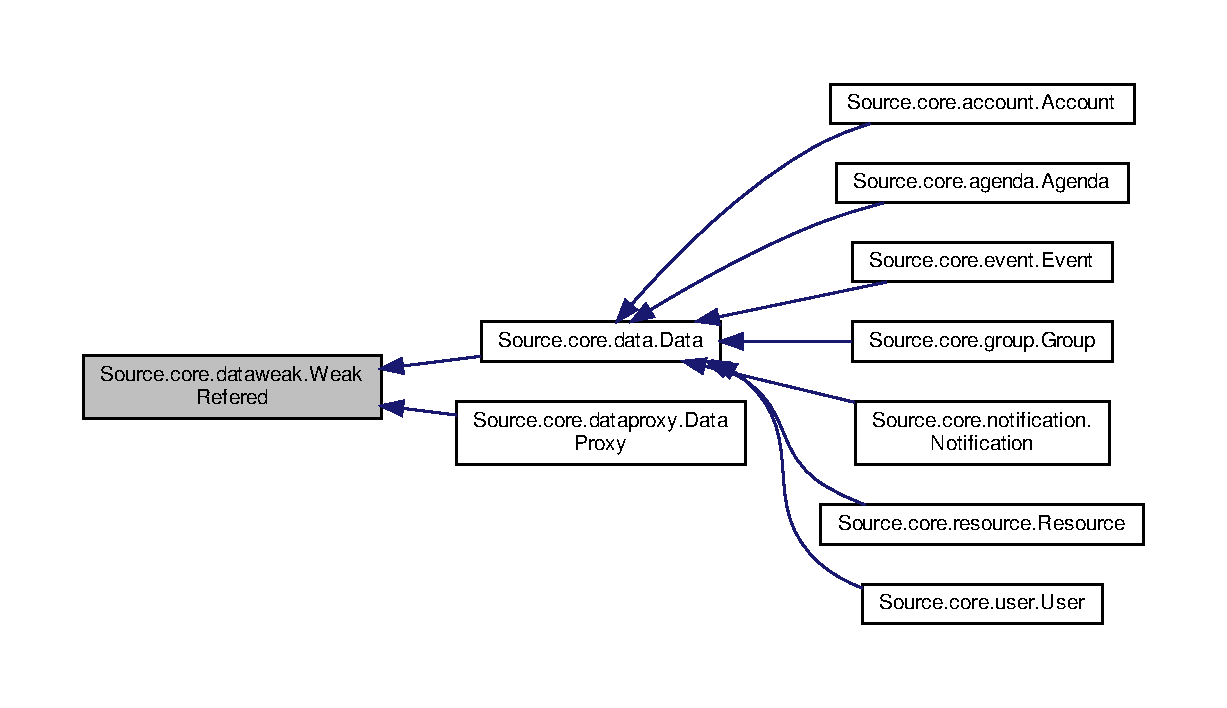
\includegraphics[width=350pt]{classSource_1_1core_1_1dataweak_1_1WeakRefered__inherit__graph}
\end{center}
\end{figure}
\subsection*{Public Member Functions}
\begin{DoxyCompactItemize}
\item 
\mbox{\Hypertarget{classSource_1_1core_1_1dataweak_1_1WeakRefered_aebf83f5d2687e065920a37fc0e60bb9f}\label{classSource_1_1core_1_1dataweak_1_1WeakRefered_aebf83f5d2687e065920a37fc0e60bb9f}} 
def {\bfseries \+\_\+\+\_\+init\+\_\+\+\_\+} (self)
\item 
\mbox{\Hypertarget{classSource_1_1core_1_1dataweak_1_1WeakRefered_a527e1d9d0a3190003d177a984fe68262}\label{classSource_1_1core_1_1dataweak_1_1WeakRefered_a527e1d9d0a3190003d177a984fe68262}} 
def {\bfseries new\+\_\+ref} (self, ref)
\item 
\mbox{\Hypertarget{classSource_1_1core_1_1dataweak_1_1WeakRefered_acc0d419f38ee8fab8be5863c5e8fdf2f}\label{classSource_1_1core_1_1dataweak_1_1WeakRefered_acc0d419f38ee8fab8be5863c5e8fdf2f}} 
def {\bfseries del\+\_\+ref} (self, ref)
\item 
\mbox{\Hypertarget{classSource_1_1core_1_1dataweak_1_1WeakRefered_aa03e59708695b4b16058fb4d9c568917}\label{classSource_1_1core_1_1dataweak_1_1WeakRefered_aa03e59708695b4b16058fb4d9c568917}} 
def {\bfseries delete} (self)
\end{DoxyCompactItemize}


The documentation for this class was generated from the following file\+:\begin{DoxyCompactItemize}
\item 
/home/tristan/\+Documents/\+U\+S\+M\+B/\+I\+N\+F\+O\+\_\+406/\+Source/core/dataweak.\+py\end{DoxyCompactItemize}

\hypertarget{classSource_1_1core_1_1dataweak_1_1WeakRefSet}{}\section{Source.\+core.\+dataweak.\+Weak\+Ref\+Set Class Reference}
\label{classSource_1_1core_1_1dataweak_1_1WeakRefSet}\index{Source.\+core.\+dataweak.\+Weak\+Ref\+Set@{Source.\+core.\+dataweak.\+Weak\+Ref\+Set}}
\subsection*{Public Member Functions}
\begin{DoxyCompactItemize}
\item 
\mbox{\Hypertarget{classSource_1_1core_1_1dataweak_1_1WeakRefSet_afd9431b29def930ddae6975f5625ca39}\label{classSource_1_1core_1_1dataweak_1_1WeakRefSet_afd9431b29def930ddae6975f5625ca39}} 
def {\bfseries \+\_\+\+\_\+init\+\_\+\+\_\+} (self, items=set(), owner=None)
\item 
\mbox{\Hypertarget{classSource_1_1core_1_1dataweak_1_1WeakRefSet_a5fc0a1d613fb3705d3db158a5d91960d}\label{classSource_1_1core_1_1dataweak_1_1WeakRefSet_a5fc0a1d613fb3705d3db158a5d91960d}} 
def {\bfseries \+\_\+\+\_\+iter\+\_\+\+\_\+} (self)
\item 
\mbox{\Hypertarget{classSource_1_1core_1_1dataweak_1_1WeakRefSet_a43ae058f44c3e6914acf1099282fb91d}\label{classSource_1_1core_1_1dataweak_1_1WeakRefSet_a43ae058f44c3e6914acf1099282fb91d}} 
def {\bfseries \+\_\+\+\_\+repr\+\_\+\+\_\+} (self)
\item 
\mbox{\Hypertarget{classSource_1_1core_1_1dataweak_1_1WeakRefSet_a8661da89878bd538d874f8a20f874419}\label{classSource_1_1core_1_1dataweak_1_1WeakRefSet_a8661da89878bd538d874f8a20f874419}} 
def {\bfseries \+\_\+\+\_\+len\+\_\+\+\_\+} (self)
\item 
\mbox{\Hypertarget{classSource_1_1core_1_1dataweak_1_1WeakRefSet_a97b08b11a22cbf66919af37fcedac381}\label{classSource_1_1core_1_1dataweak_1_1WeakRefSet_a97b08b11a22cbf66919af37fcedac381}} 
def {\bfseries \+\_\+\+\_\+ior\+\_\+\+\_\+} (self, other)
\item 
\mbox{\Hypertarget{classSource_1_1core_1_1dataweak_1_1WeakRefSet_ab8919c1838c75617f728e017b8615a70}\label{classSource_1_1core_1_1dataweak_1_1WeakRefSet_ab8919c1838c75617f728e017b8615a70}} 
def {\bfseries \+\_\+\+\_\+rsub\+\_\+\+\_\+} (self, other)
\item 
\mbox{\Hypertarget{classSource_1_1core_1_1dataweak_1_1WeakRefSet_a303e3078fe9049ad8909c6d2c4bd5c23}\label{classSource_1_1core_1_1dataweak_1_1WeakRefSet_a303e3078fe9049ad8909c6d2c4bd5c23}} 
def {\bfseries delete} (self, refered)
\item 
\mbox{\Hypertarget{classSource_1_1core_1_1dataweak_1_1WeakRefSet_a01c976e2adf037210a018f1d4b5d2558}\label{classSource_1_1core_1_1dataweak_1_1WeakRefSet_a01c976e2adf037210a018f1d4b5d2558}} 
def {\bfseries discard} (self, item)
\item 
\mbox{\Hypertarget{classSource_1_1core_1_1dataweak_1_1WeakRefSet_a1586db17918bf67f3cbd54ba6cd8932b}\label{classSource_1_1core_1_1dataweak_1_1WeakRefSet_a1586db17918bf67f3cbd54ba6cd8932b}} 
def {\bfseries add} (self, item)
\end{DoxyCompactItemize}
\subsection*{Public Attributes}
\begin{DoxyCompactItemize}
\item 
\mbox{\Hypertarget{classSource_1_1core_1_1dataweak_1_1WeakRefSet_aad79e1c6ef86604ddbad56c37bc896bb}\label{classSource_1_1core_1_1dataweak_1_1WeakRefSet_aad79e1c6ef86604ddbad56c37bc896bb}} 
{\bfseries owner}
\end{DoxyCompactItemize}


The documentation for this class was generated from the following file\+:\begin{DoxyCompactItemize}
\item 
/home/tristan/\+Documents/\+U\+S\+M\+B/\+I\+N\+F\+O\+\_\+406/\+Source/core/dataweak.\+py\end{DoxyCompactItemize}

%--- End generated contents ---

% Index
\backmatter
\newpage
\phantomsection
\clearemptydoublepage
\addcontentsline{toc}{chapter}{Index}
\printindex

\end{document}
